\documentclass[twoside]{book}

% Packages required by doxygen
\usepackage{fixltx2e}
\usepackage{calc}
\usepackage{doxygen}
\usepackage[export]{adjustbox} % also loads graphicx
\usepackage{graphicx}
\usepackage[utf8]{inputenc}
\usepackage{makeidx}
\usepackage{multicol}
\usepackage{multirow}
\PassOptionsToPackage{warn}{textcomp}
\usepackage{textcomp}
\usepackage[nointegrals]{wasysym}
\usepackage[table]{xcolor}

% Font selection
\usepackage[T1]{fontenc}
\usepackage[scaled=.90]{helvet}
\usepackage{courier}
\usepackage{amssymb}
\usepackage{sectsty}
\renewcommand{\familydefault}{\sfdefault}
\allsectionsfont{%
  \fontseries{bc}\selectfont%
  \color{darkgray}%
}
\renewcommand{\DoxyLabelFont}{%
  \fontseries{bc}\selectfont%
  \color{darkgray}%
}
\newcommand{\+}{\discretionary{\mbox{\scriptsize$\hookleftarrow$}}{}{}}

% Page & text layout
\usepackage{geometry}
\geometry{%
  a4paper,%
  top=2.5cm,%
  bottom=2.5cm,%
  left=2.5cm,%
  right=2.5cm%
}
\tolerance=750
\hfuzz=15pt
\hbadness=750
\setlength{\emergencystretch}{15pt}
\setlength{\parindent}{0cm}
\setlength{\parskip}{3ex plus 2ex minus 2ex}
\makeatletter
\renewcommand{\paragraph}{%
  \@startsection{paragraph}{4}{0ex}{-1.0ex}{1.0ex}{%
    \normalfont\normalsize\bfseries\SS@parafont%
  }%
}
\renewcommand{\subparagraph}{%
  \@startsection{subparagraph}{5}{0ex}{-1.0ex}{1.0ex}{%
    \normalfont\normalsize\bfseries\SS@subparafont%
  }%
}
\makeatother

% Headers & footers
\usepackage{fancyhdr}
\pagestyle{fancyplain}
\fancyhead[LE]{\fancyplain{}{\bfseries\thepage}}
\fancyhead[CE]{\fancyplain{}{}}
\fancyhead[RE]{\fancyplain{}{\bfseries\leftmark}}
\fancyhead[LO]{\fancyplain{}{\bfseries\rightmark}}
\fancyhead[CO]{\fancyplain{}{}}
\fancyhead[RO]{\fancyplain{}{\bfseries\thepage}}
\fancyfoot[LE]{\fancyplain{}{}}
\fancyfoot[CE]{\fancyplain{}{}}
\fancyfoot[RE]{\fancyplain{}{\bfseries\scriptsize Generated by Doxygen }}
\fancyfoot[LO]{\fancyplain{}{\bfseries\scriptsize Generated by Doxygen }}
\fancyfoot[CO]{\fancyplain{}{}}
\fancyfoot[RO]{\fancyplain{}{}}
\renewcommand{\footrulewidth}{0.4pt}
\renewcommand{\chaptermark}[1]{%
  \markboth{#1}{}%
}
\renewcommand{\sectionmark}[1]{%
  \markright{\thesection\ #1}%
}

% Indices & bibliography
\usepackage{natbib}
\usepackage[titles]{tocloft}
\setcounter{tocdepth}{3}
\setcounter{secnumdepth}{5}
\makeindex

% Hyperlinks (required, but should be loaded last)
\usepackage{ifpdf}
\ifpdf
  \usepackage[pdftex,pagebackref=true]{hyperref}
\else
  \usepackage[ps2pdf,pagebackref=true]{hyperref}
\fi
\hypersetup{%
  colorlinks=true,%
  linkcolor=blue,%
  citecolor=blue,%
  unicode%
}

% Custom commands
\newcommand{\clearemptydoublepage}{%
  \newpage{\pagestyle{empty}\cleardoublepage}%
}

\usepackage{caption}
\captionsetup{labelsep=space,justification=centering,font={bf},singlelinecheck=off,skip=4pt,position=top}

%===== C O N T E N T S =====

\begin{document}

% Titlepage & ToC
\hypersetup{pageanchor=false,
             bookmarksnumbered=true,
             pdfencoding=unicode
            }
\pagenumbering{alph}
\begin{titlepage}
\vspace*{7cm}
\begin{center}%
{\Large c2 -\/ projekt }\\
\vspace*{1cm}
{\large Generated by Doxygen 1.8.13}\\
\end{center}
\end{titlepage}
\clearemptydoublepage
\pagenumbering{roman}
\tableofcontents
\clearemptydoublepage
\pagenumbering{arabic}
\hypersetup{pageanchor=true}

%--- Begin generated contents ---
\chapter{Hierarchical Index}
\section{Class Hierarchy}
This inheritance list is sorted roughly, but not completely, alphabetically\+:\begin{DoxyCompactList}
\item \contentsline{section}{Abstract\+Map\+Block}{\pageref{class_abstract_map_block}}{}
\begin{DoxyCompactList}
\item \contentsline{section}{Block}{\pageref{class_block}}{}
\item \contentsline{section}{Bridge\+Block}{\pageref{class_bridge_block}}{}
\item \contentsline{section}{Bush\+Block}{\pageref{class_bush_block}}{}
\item \contentsline{section}{Crate\+Block}{\pageref{class_crate_block}}{}
\item \contentsline{section}{Ground\+Block}{\pageref{class_ground_block}}{}
\item \contentsline{section}{Plank\+Block}{\pageref{class_plank_block}}{}
\item \contentsline{section}{Spikes\+Block}{\pageref{class_spikes_block}}{}
\item \contentsline{section}{Stone\+Block}{\pageref{class_stone_block}}{}
\end{DoxyCompactList}
\item \contentsline{section}{Character}{\pageref{class_character}}{}
\item \contentsline{section}{Display\+Map\+Manager}{\pageref{class_display_map_manager}}{}
\item \contentsline{section}{Gravity}{\pageref{class_gravity}}{}
\item \contentsline{section}{H\+UD}{\pageref{class_h_u_d}}{}
\item \contentsline{section}{Map}{\pageref{class_map}}{}
\end{DoxyCompactList}

\chapter{Class Index}
\section{Class List}
Here are the classes, structs, unions and interfaces with brief descriptions\+:\begin{DoxyCompactList}
\item\contentsline{section}{\hyperlink{class_abstract_map_block}{Abstract\+Map\+Block} }{\pageref{class_abstract_map_block}}{}
\item\contentsline{section}{\hyperlink{class_block}{Block} }{\pageref{class_block}}{}
\item\contentsline{section}{\hyperlink{class_bridge_block}{Bridge\+Block} }{\pageref{class_bridge_block}}{}
\item\contentsline{section}{\hyperlink{class_bush_block}{Bush\+Block} }{\pageref{class_bush_block}}{}
\item\contentsline{section}{\hyperlink{class_character}{Character} }{\pageref{class_character}}{}
\item\contentsline{section}{\hyperlink{class_crate_block}{Crate\+Block} }{\pageref{class_crate_block}}{}
\item\contentsline{section}{\hyperlink{class_display_map_manager}{Display\+Map\+Manager} }{\pageref{class_display_map_manager}}{}
\item\contentsline{section}{\hyperlink{class_gravity}{Gravity} }{\pageref{class_gravity}}{}
\item\contentsline{section}{\hyperlink{class_ground_block}{Ground\+Block} }{\pageref{class_ground_block}}{}
\item\contentsline{section}{\hyperlink{class_h_u_d}{H\+UD} }{\pageref{class_h_u_d}}{}
\item\contentsline{section}{\hyperlink{class_map}{Map} }{\pageref{class_map}}{}
\item\contentsline{section}{\hyperlink{class_plank_block}{Plank\+Block} }{\pageref{class_plank_block}}{}
\item\contentsline{section}{\hyperlink{class_spikes_block}{Spikes\+Block} }{\pageref{class_spikes_block}}{}
\item\contentsline{section}{\hyperlink{class_stone_block}{Stone\+Block} }{\pageref{class_stone_block}}{}
\end{DoxyCompactList}

\chapter{File Index}
\section{File List}
Here is a list of all files with brief descriptions\+:\begin{DoxyCompactList}
\item\contentsline{section}{\hyperlink{_abstract_map_block_8cpp}{Abstract\+Map\+Block.\+cpp} }{\pageref{_abstract_map_block_8cpp}}{}
\item\contentsline{section}{\hyperlink{_abstract_map_block_8h}{Abstract\+Map\+Block.\+h} }{\pageref{_abstract_map_block_8h}}{}
\item\contentsline{section}{\hyperlink{_block_8cpp}{Block.\+cpp} }{\pageref{_block_8cpp}}{}
\item\contentsline{section}{\hyperlink{_block_8h}{Block.\+h} }{\pageref{_block_8h}}{}
\item\contentsline{section}{\hyperlink{_bridge_block_8cpp}{Bridge\+Block.\+cpp} }{\pageref{_bridge_block_8cpp}}{}
\item\contentsline{section}{\hyperlink{_bridge_block_8h}{Bridge\+Block.\+h} }{\pageref{_bridge_block_8h}}{}
\item\contentsline{section}{\hyperlink{_bush_block_8cpp}{Bush\+Block.\+cpp} }{\pageref{_bush_block_8cpp}}{}
\item\contentsline{section}{\hyperlink{_bush_block_8h}{Bush\+Block.\+h} }{\pageref{_bush_block_8h}}{}
\item\contentsline{section}{\hyperlink{c2_project_8cpp}{c2\+Project.\+cpp} }{\pageref{c2_project_8cpp}}{}
\item\contentsline{section}{\hyperlink{_character_8cpp}{Character.\+cpp} }{\pageref{_character_8cpp}}{}
\item\contentsline{section}{\hyperlink{_character_8h}{Character.\+h} }{\pageref{_character_8h}}{}
\item\contentsline{section}{\hyperlink{_crate_block_8cpp}{Crate\+Block.\+cpp} }{\pageref{_crate_block_8cpp}}{}
\item\contentsline{section}{\hyperlink{_crate_block_8h}{Crate\+Block.\+h} }{\pageref{_crate_block_8h}}{}
\item\contentsline{section}{\hyperlink{_display_map_manager_8cpp}{Display\+Map\+Manager.\+cpp} }{\pageref{_display_map_manager_8cpp}}{}
\item\contentsline{section}{\hyperlink{_display_map_manager_8h}{Display\+Map\+Manager.\+h} }{\pageref{_display_map_manager_8h}}{}
\item\contentsline{section}{\hyperlink{_gravity_8cpp}{Gravity.\+cpp} }{\pageref{_gravity_8cpp}}{}
\item\contentsline{section}{\hyperlink{_gravity_8h}{Gravity.\+h} }{\pageref{_gravity_8h}}{}
\item\contentsline{section}{\hyperlink{_ground_block_8cpp}{Ground\+Block.\+cpp} }{\pageref{_ground_block_8cpp}}{}
\item\contentsline{section}{\hyperlink{_ground_block_8h}{Ground\+Block.\+h} }{\pageref{_ground_block_8h}}{}
\item\contentsline{section}{\hyperlink{_map_8cpp}{Map.\+cpp} }{\pageref{_map_8cpp}}{}
\item\contentsline{section}{\hyperlink{_map_8h}{Map.\+h} }{\pageref{_map_8h}}{}
\item\contentsline{section}{\hyperlink{_plank_block_8cpp}{Plank\+Block.\+cpp} }{\pageref{_plank_block_8cpp}}{}
\item\contentsline{section}{\hyperlink{_plank_block_8h}{Plank\+Block.\+h} }{\pageref{_plank_block_8h}}{}
\item\contentsline{section}{\hyperlink{resource_8h}{resource.\+h} }{\pageref{resource_8h}}{}
\item\contentsline{section}{\hyperlink{_spikes_block_8cpp}{Spikes\+Block.\+cpp} }{\pageref{_spikes_block_8cpp}}{}
\item\contentsline{section}{\hyperlink{_spikes_block_8h}{Spikes\+Block.\+h} }{\pageref{_spikes_block_8h}}{}
\item\contentsline{section}{\hyperlink{stdafx_8cpp}{stdafx.\+cpp} }{\pageref{stdafx_8cpp}}{}
\item\contentsline{section}{\hyperlink{stdafx_8h}{stdafx.\+h} }{\pageref{stdafx_8h}}{}
\item\contentsline{section}{\hyperlink{_stone_block_8cpp}{Stone\+Block.\+cpp} }{\pageref{_stone_block_8cpp}}{}
\item\contentsline{section}{\hyperlink{_stone_block_8h}{Stone\+Block.\+h} }{\pageref{_stone_block_8h}}{}
\item\contentsline{section}{\hyperlink{targetver_8h}{targetver.\+h} }{\pageref{targetver_8h}}{}
\end{DoxyCompactList}

\chapter{Class Documentation}
\hypertarget{class_abstract_map_block}{}\section{Abstract\+Map\+Block Class Reference}
\label{class_abstract_map_block}\index{Abstract\+Map\+Block@{Abstract\+Map\+Block}}


{\ttfamily \#include $<$Abstract\+Map\+Block.\+h$>$}

Inheritance diagram for Abstract\+Map\+Block\+:\begin{figure}[H]
\begin{center}
\leavevmode
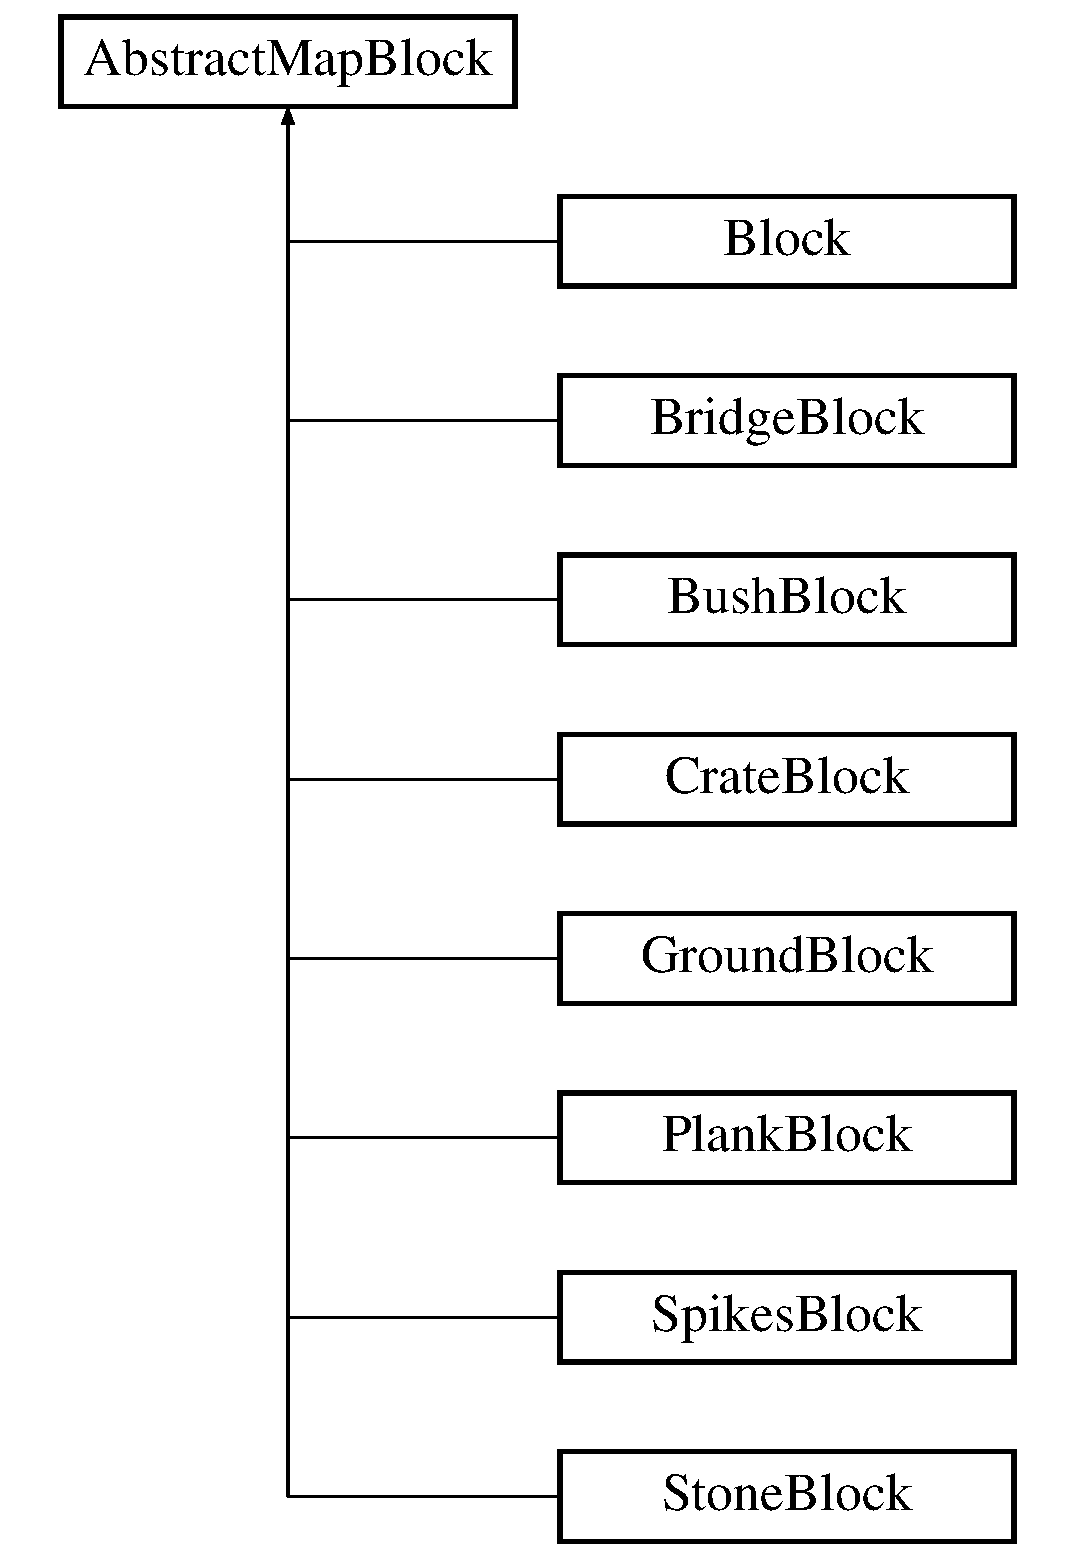
\includegraphics[height=9.000000cm]{class_abstract_map_block}
\end{center}
\end{figure}
\subsection*{Public Member Functions}
\begin{DoxyCompactItemize}
\item 
\mbox{\Hypertarget{class_abstract_map_block_afea0f904a49f56b417387f721c8677c9}\label{class_abstract_map_block_afea0f904a49f56b417387f721c8677c9}} 
{\bfseries Abstract\+Map\+Block} (int x, int y)
\item 
\mbox{\Hypertarget{class_abstract_map_block_ab5a448a1b6478d10a8814c6d19c4fdb4}\label{class_abstract_map_block_ab5a448a1b6478d10a8814c6d19c4fdb4}} 
virtual sf\+::\+Sprite $\ast$ {\bfseries get\+Sprite} ()=0
\end{DoxyCompactItemize}
\subsection*{Public Attributes}
\begin{DoxyCompactItemize}
\item 
\mbox{\Hypertarget{class_abstract_map_block_afdfb3d8630fb089667c05daa27598ebb}\label{class_abstract_map_block_afdfb3d8630fb089667c05daa27598ebb}} 
int {\bfseries width} = 25
\item 
\mbox{\Hypertarget{class_abstract_map_block_ac20fe00ed32681d06378dd62e5901092}\label{class_abstract_map_block_ac20fe00ed32681d06378dd62e5901092}} 
int {\bfseries height} = 25
\item 
\mbox{\Hypertarget{class_abstract_map_block_a5aa7d9d05727ac3b0f0f4746813d77e7}\label{class_abstract_map_block_a5aa7d9d05727ac3b0f0f4746813d77e7}} 
int {\bfseries posX} = 0
\item 
\mbox{\Hypertarget{class_abstract_map_block_a5e286fbe867af6c78c17e7e21f9948c4}\label{class_abstract_map_block_a5e286fbe867af6c78c17e7e21f9948c4}} 
int {\bfseries posY} = 0
\item 
\mbox{\Hypertarget{class_abstract_map_block_ae4151be3ea8a899aa9423e57262ef93e}\label{class_abstract_map_block_ae4151be3ea8a899aa9423e57262ef93e}} 
bool {\bfseries is\+Wall} = true
\end{DoxyCompactItemize}


\subsection{Detailed Description}
Abstrakcyjna klasa bloku, po ktorej dziedzicza wszystkie mozliwe elementy ktore mozna umiescic na mapie 

The documentation for this class was generated from the following files\+:\begin{DoxyCompactItemize}
\item 
Abstract\+Map\+Block.\+h\item 
Abstract\+Map\+Block.\+cpp\end{DoxyCompactItemize}

\hypertarget{class_block}{}\section{Block Class Reference}
\label{class_block}\index{Block@{Block}}


{\ttfamily \#include $<$Block.\+h$>$}

Inheritance diagram for Block\+:\begin{figure}[H]
\begin{center}
\leavevmode
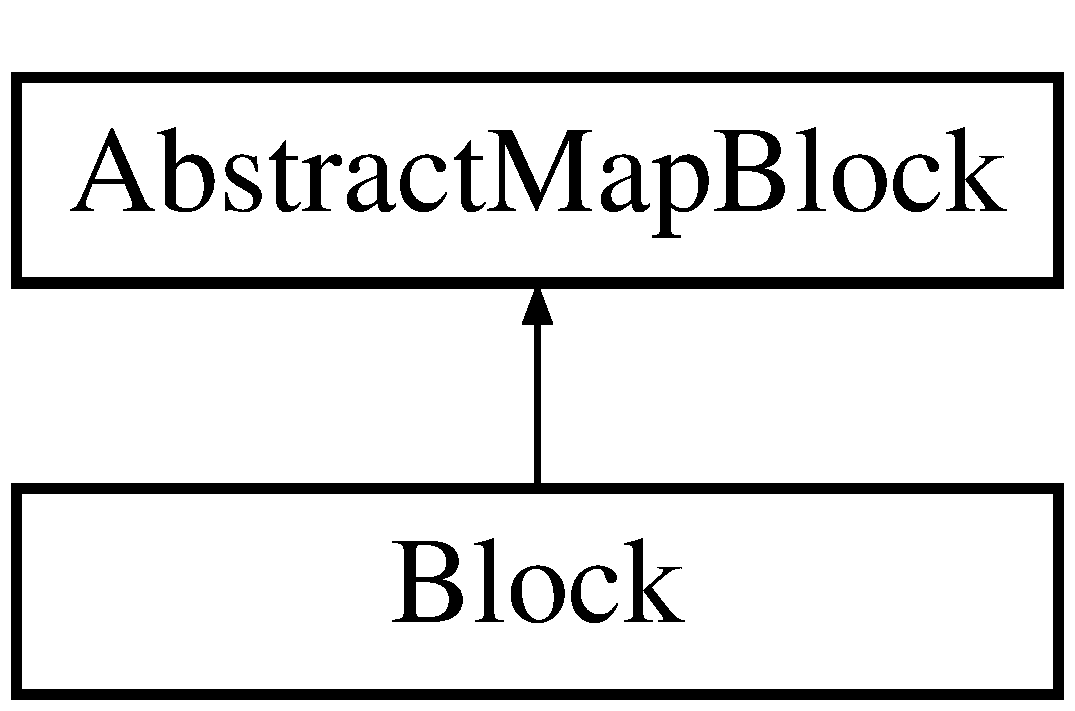
\includegraphics[height=2.000000cm]{class_block}
\end{center}
\end{figure}
\subsection*{Public Member Functions}
\begin{DoxyCompactItemize}
\item 
\hyperlink{class_block_a37658a946bf5067ad01d68d9ff086adc}{Block} ()
\item 
\hyperlink{class_block_a3ff2925a4aa73cb9cabe5097b79f636e}{Block} (int x, int y)
\item 
\hyperlink{class_block_a19d1bd0e1cef6a865ed2745a2e648405}{$\sim$\+Block} ()
\item 
sf\+::\+Sprite $\ast$ \hyperlink{class_block_acd9b061af3ad9e79cf49bf9d4dc3d8b9}{get\+Sprite} ()
\end{DoxyCompactItemize}
\subsection*{Protected Attributes}
\begin{DoxyCompactItemize}
\item 
sf\+::\+Texture $\ast$ \hyperlink{class_block_a61ef2e4fef4ab4a950d3217f88cb8369}{texture}
\item 
sf\+::\+Sprite $\ast$ \hyperlink{class_block_a5cf88ebac5cc92a309ec3e0d9c9d5fe8}{sprite}
\end{DoxyCompactItemize}
\subsection*{Additional Inherited Members}


\subsection{Detailed Description}
Blok reprezentujacy zwykly bloczek w grze, nie spelniajacy zadnych specjalnych funkcji 

\subsection{Constructor \& Destructor Documentation}
\mbox{\Hypertarget{class_block_a37658a946bf5067ad01d68d9ff086adc}\label{class_block_a37658a946bf5067ad01d68d9ff086adc}} 
\index{Block@{Block}!Block@{Block}}
\index{Block@{Block}!Block@{Block}}
\subsubsection{\texorpdfstring{Block()}{Block()}\hspace{0.1cm}{\footnotesize\ttfamily [1/2]}}
{\footnotesize\ttfamily Block\+::\+Block (\begin{DoxyParamCaption}{ }\end{DoxyParamCaption})}

Konstruktr bez parametrow, nie moze byc wywolywany! \mbox{\Hypertarget{class_block_a3ff2925a4aa73cb9cabe5097b79f636e}\label{class_block_a3ff2925a4aa73cb9cabe5097b79f636e}} 
\index{Block@{Block}!Block@{Block}}
\index{Block@{Block}!Block@{Block}}
\subsubsection{\texorpdfstring{Block()}{Block()}\hspace{0.1cm}{\footnotesize\ttfamily [2/2]}}
{\footnotesize\ttfamily Block\+::\+Block (\begin{DoxyParamCaption}\item[{int}]{x,  }\item[{int}]{y }\end{DoxyParamCaption})}

\mbox{\Hypertarget{class_block_a19d1bd0e1cef6a865ed2745a2e648405}\label{class_block_a19d1bd0e1cef6a865ed2745a2e648405}} 
\index{Block@{Block}!````~Block@{$\sim$\+Block}}
\index{````~Block@{$\sim$\+Block}!Block@{Block}}
\subsubsection{\texorpdfstring{$\sim$\+Block()}{~Block()}}
{\footnotesize\ttfamily Block\+::$\sim$\+Block (\begin{DoxyParamCaption}{ }\end{DoxyParamCaption})}

Destruktor 

\subsection{Member Function Documentation}
\mbox{\Hypertarget{class_block_acd9b061af3ad9e79cf49bf9d4dc3d8b9}\label{class_block_acd9b061af3ad9e79cf49bf9d4dc3d8b9}} 
\index{Block@{Block}!get\+Sprite@{get\+Sprite}}
\index{get\+Sprite@{get\+Sprite}!Block@{Block}}
\subsubsection{\texorpdfstring{get\+Sprite()}{getSprite()}}
{\footnotesize\ttfamily sf\+::\+Sprite $\ast$ Block\+::get\+Sprite (\begin{DoxyParamCaption}{ }\end{DoxyParamCaption})\hspace{0.3cm}{\ttfamily [virtual]}}

zwraca sprite-\/a 

Implements \hyperlink{class_abstract_map_block_ab5a448a1b6478d10a8814c6d19c4fdb4}{Abstract\+Map\+Block}.



\subsection{Member Data Documentation}
\mbox{\Hypertarget{class_block_a5cf88ebac5cc92a309ec3e0d9c9d5fe8}\label{class_block_a5cf88ebac5cc92a309ec3e0d9c9d5fe8}} 
\index{Block@{Block}!sprite@{sprite}}
\index{sprite@{sprite}!Block@{Block}}
\subsubsection{\texorpdfstring{sprite}{sprite}}
{\footnotesize\ttfamily sf\+::\+Sprite$\ast$ Block\+::sprite\hspace{0.3cm}{\ttfamily [protected]}}

Sprite danego bloku \mbox{\Hypertarget{class_block_a61ef2e4fef4ab4a950d3217f88cb8369}\label{class_block_a61ef2e4fef4ab4a950d3217f88cb8369}} 
\index{Block@{Block}!texture@{texture}}
\index{texture@{texture}!Block@{Block}}
\subsubsection{\texorpdfstring{texture}{texture}}
{\footnotesize\ttfamily sf\+::\+Texture$\ast$ Block\+::texture\hspace{0.3cm}{\ttfamily [protected]}}

Tekstura danego bloku 

The documentation for this class was generated from the following files\+:\begin{DoxyCompactItemize}
\item 
\hyperlink{_block_8h}{Block.\+h}\item 
\hyperlink{_block_8cpp}{Block.\+cpp}\end{DoxyCompactItemize}

\hypertarget{class_bridge_block}{}\section{Bridge\+Block Class Reference}
\label{class_bridge_block}\index{Bridge\+Block@{Bridge\+Block}}


{\ttfamily \#include $<$Bridge\+Block.\+h$>$}

Inheritance diagram for Bridge\+Block\+:\begin{figure}[H]
\begin{center}
\leavevmode
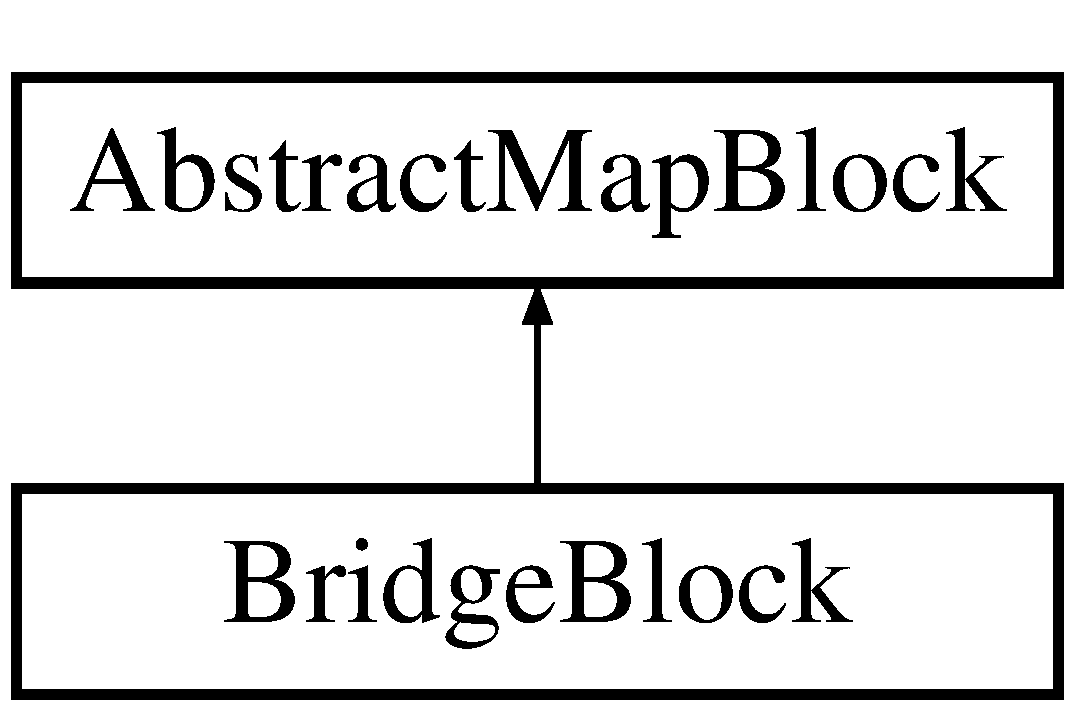
\includegraphics[height=2.000000cm]{class_bridge_block}
\end{center}
\end{figure}
\subsection*{Public Member Functions}
\begin{DoxyCompactItemize}
\item 
\hyperlink{class_bridge_block_a3a383311a5e2472e435c1633eeccab3d}{Bridge\+Block} ()
\item 
\hyperlink{class_bridge_block_a17bb807971dbc0b222a27e6bd18a9085}{Bridge\+Block} (int x, int y)
\item 
\hyperlink{class_bridge_block_a56ad5e506bc091b779289a053bf45393}{$\sim$\+Bridge\+Block} ()
\item 
sf\+::\+Sprite $\ast$ \hyperlink{class_bridge_block_a6ea5fa76b21c9805702c7f214e661198}{get\+Sprite} ()
\end{DoxyCompactItemize}
\subsection*{Protected Attributes}
\begin{DoxyCompactItemize}
\item 
sf\+::\+Texture $\ast$ \hyperlink{class_bridge_block_aeab425af654b8ae2edc7ba29421fe5b0}{texture}
\item 
sf\+::\+Sprite $\ast$ \hyperlink{class_bridge_block_a93817188870fb7eb4137a90a7025a748}{sprite}
\end{DoxyCompactItemize}
\subsection*{Additional Inherited Members}


\subsection{Detailed Description}
Blok reprezentujacy drewniany mostek w grze 

\subsection{Constructor \& Destructor Documentation}
\mbox{\Hypertarget{class_bridge_block_a3a383311a5e2472e435c1633eeccab3d}\label{class_bridge_block_a3a383311a5e2472e435c1633eeccab3d}} 
\index{Bridge\+Block@{Bridge\+Block}!Bridge\+Block@{Bridge\+Block}}
\index{Bridge\+Block@{Bridge\+Block}!Bridge\+Block@{Bridge\+Block}}
\subsubsection{\texorpdfstring{Bridge\+Block()}{BridgeBlock()}\hspace{0.1cm}{\footnotesize\ttfamily [1/2]}}
{\footnotesize\ttfamily Bridge\+Block\+::\+Bridge\+Block (\begin{DoxyParamCaption}{ }\end{DoxyParamCaption})}

Konstruktr bez parametrow, nie moze byc wywolywany! \mbox{\Hypertarget{class_bridge_block_a17bb807971dbc0b222a27e6bd18a9085}\label{class_bridge_block_a17bb807971dbc0b222a27e6bd18a9085}} 
\index{Bridge\+Block@{Bridge\+Block}!Bridge\+Block@{Bridge\+Block}}
\index{Bridge\+Block@{Bridge\+Block}!Bridge\+Block@{Bridge\+Block}}
\subsubsection{\texorpdfstring{Bridge\+Block()}{BridgeBlock()}\hspace{0.1cm}{\footnotesize\ttfamily [2/2]}}
{\footnotesize\ttfamily Bridge\+Block\+::\+Bridge\+Block (\begin{DoxyParamCaption}\item[{int}]{x,  }\item[{int}]{y }\end{DoxyParamCaption})}

Konstruktr, z parametrami x i y danego bloku, wzgledem mapy \mbox{\Hypertarget{class_bridge_block_a56ad5e506bc091b779289a053bf45393}\label{class_bridge_block_a56ad5e506bc091b779289a053bf45393}} 
\index{Bridge\+Block@{Bridge\+Block}!````~Bridge\+Block@{$\sim$\+Bridge\+Block}}
\index{````~Bridge\+Block@{$\sim$\+Bridge\+Block}!Bridge\+Block@{Bridge\+Block}}
\subsubsection{\texorpdfstring{$\sim$\+Bridge\+Block()}{~BridgeBlock()}}
{\footnotesize\ttfamily Bridge\+Block\+::$\sim$\+Bridge\+Block (\begin{DoxyParamCaption}{ }\end{DoxyParamCaption})}

Destruktor 

\subsection{Member Function Documentation}
\mbox{\Hypertarget{class_bridge_block_a6ea5fa76b21c9805702c7f214e661198}\label{class_bridge_block_a6ea5fa76b21c9805702c7f214e661198}} 
\index{Bridge\+Block@{Bridge\+Block}!get\+Sprite@{get\+Sprite}}
\index{get\+Sprite@{get\+Sprite}!Bridge\+Block@{Bridge\+Block}}
\subsubsection{\texorpdfstring{get\+Sprite()}{getSprite()}}
{\footnotesize\ttfamily sf\+::\+Sprite $\ast$ Bridge\+Block\+::get\+Sprite (\begin{DoxyParamCaption}{ }\end{DoxyParamCaption})\hspace{0.3cm}{\ttfamily [virtual]}}

zwraca sprite-\/a 

Implements \hyperlink{class_abstract_map_block_ab5a448a1b6478d10a8814c6d19c4fdb4}{Abstract\+Map\+Block}.



\subsection{Member Data Documentation}
\mbox{\Hypertarget{class_bridge_block_a93817188870fb7eb4137a90a7025a748}\label{class_bridge_block_a93817188870fb7eb4137a90a7025a748}} 
\index{Bridge\+Block@{Bridge\+Block}!sprite@{sprite}}
\index{sprite@{sprite}!Bridge\+Block@{Bridge\+Block}}
\subsubsection{\texorpdfstring{sprite}{sprite}}
{\footnotesize\ttfamily sf\+::\+Sprite$\ast$ Bridge\+Block\+::sprite\hspace{0.3cm}{\ttfamily [protected]}}

Sprite danego bloku \mbox{\Hypertarget{class_bridge_block_aeab425af654b8ae2edc7ba29421fe5b0}\label{class_bridge_block_aeab425af654b8ae2edc7ba29421fe5b0}} 
\index{Bridge\+Block@{Bridge\+Block}!texture@{texture}}
\index{texture@{texture}!Bridge\+Block@{Bridge\+Block}}
\subsubsection{\texorpdfstring{texture}{texture}}
{\footnotesize\ttfamily sf\+::\+Texture$\ast$ Bridge\+Block\+::texture\hspace{0.3cm}{\ttfamily [protected]}}

Tekstura danego bloku 

The documentation for this class was generated from the following files\+:\begin{DoxyCompactItemize}
\item 
\hyperlink{_bridge_block_8h}{Bridge\+Block.\+h}\item 
\hyperlink{_bridge_block_8cpp}{Bridge\+Block.\+cpp}\end{DoxyCompactItemize}

\hypertarget{class_bush_block}{}\section{Bush\+Block Class Reference}
\label{class_bush_block}\index{Bush\+Block@{Bush\+Block}}


{\ttfamily \#include $<$Bush\+Block.\+h$>$}

Inheritance diagram for Bush\+Block\+:\begin{figure}[H]
\begin{center}
\leavevmode
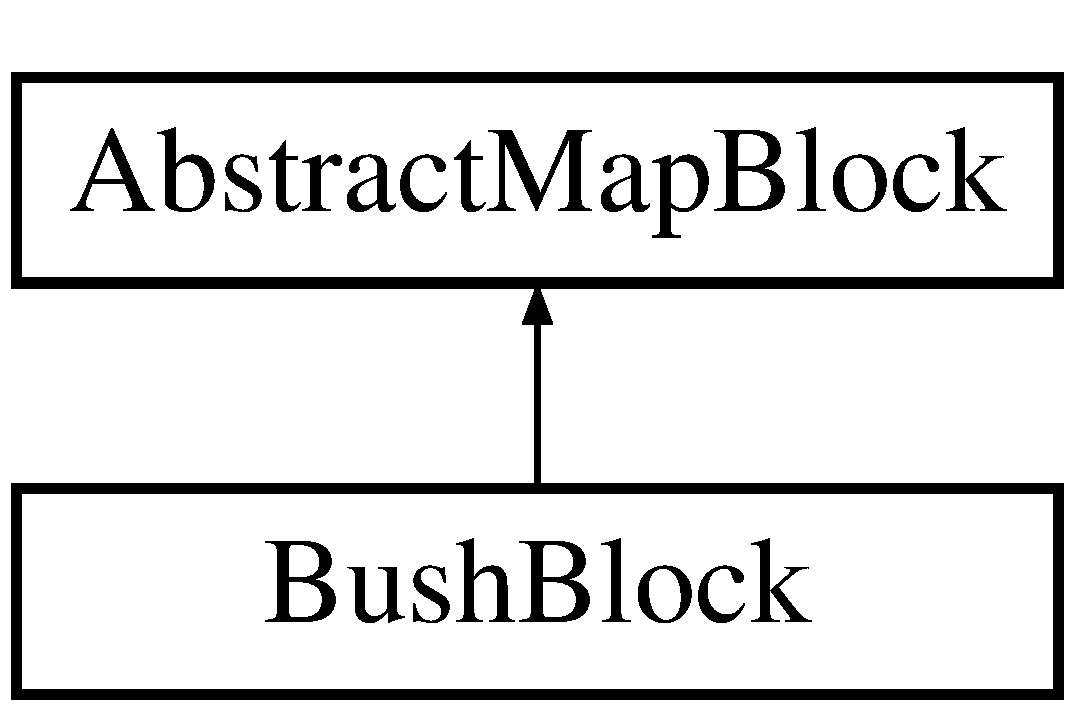
\includegraphics[height=2.000000cm]{class_bush_block}
\end{center}
\end{figure}
\subsection*{Public Member Functions}
\begin{DoxyCompactItemize}
\item 
\hyperlink{class_bush_block_a866cb791101f70cd89795b0de45c041b}{Bush\+Block} ()
\item 
\hyperlink{class_bush_block_a27d102ac30e12c537e6a8de34ce50779}{Bush\+Block} (int x, int y)
\item 
\hyperlink{class_bush_block_acffc1c20ebfc301e3c9b99912b20c5e2}{$\sim$\+Bush\+Block} ()
\item 
sf\+::\+Sprite $\ast$ \hyperlink{class_bush_block_ac6346ab038665e207134bb68ab3f20a1}{get\+Sprite} ()
\end{DoxyCompactItemize}
\subsection*{Protected Attributes}
\begin{DoxyCompactItemize}
\item 
sf\+::\+Texture $\ast$ \hyperlink{class_bush_block_af04c47ff2490b42258b0b56a6dc1aabe}{texture}
\item 
sf\+::\+Sprite $\ast$ \hyperlink{class_bush_block_a24bfc3a63232d1466d9c5ddb7459cf55}{sprite}
\end{DoxyCompactItemize}
\subsection*{Additional Inherited Members}


\subsection{Detailed Description}
Blok reprezentujacy krzak w grze, przez ktory gracz moze przechodzic (pojawia sie w tle) 

\subsection{Constructor \& Destructor Documentation}
\mbox{\Hypertarget{class_bush_block_a866cb791101f70cd89795b0de45c041b}\label{class_bush_block_a866cb791101f70cd89795b0de45c041b}} 
\index{Bush\+Block@{Bush\+Block}!Bush\+Block@{Bush\+Block}}
\index{Bush\+Block@{Bush\+Block}!Bush\+Block@{Bush\+Block}}
\subsubsection{\texorpdfstring{Bush\+Block()}{BushBlock()}\hspace{0.1cm}{\footnotesize\ttfamily [1/2]}}
{\footnotesize\ttfamily Bush\+Block\+::\+Bush\+Block (\begin{DoxyParamCaption}{ }\end{DoxyParamCaption})}

Konstruktr bez parametrow, nie moze byc wywolywany! \mbox{\Hypertarget{class_bush_block_a27d102ac30e12c537e6a8de34ce50779}\label{class_bush_block_a27d102ac30e12c537e6a8de34ce50779}} 
\index{Bush\+Block@{Bush\+Block}!Bush\+Block@{Bush\+Block}}
\index{Bush\+Block@{Bush\+Block}!Bush\+Block@{Bush\+Block}}
\subsubsection{\texorpdfstring{Bush\+Block()}{BushBlock()}\hspace{0.1cm}{\footnotesize\ttfamily [2/2]}}
{\footnotesize\ttfamily Bush\+Block\+::\+Bush\+Block (\begin{DoxyParamCaption}\item[{int}]{x,  }\item[{int}]{y }\end{DoxyParamCaption})}

Konstruktr, z parametrami x i y danego bloku, wzgledem mapy \mbox{\Hypertarget{class_bush_block_acffc1c20ebfc301e3c9b99912b20c5e2}\label{class_bush_block_acffc1c20ebfc301e3c9b99912b20c5e2}} 
\index{Bush\+Block@{Bush\+Block}!````~Bush\+Block@{$\sim$\+Bush\+Block}}
\index{````~Bush\+Block@{$\sim$\+Bush\+Block}!Bush\+Block@{Bush\+Block}}
\subsubsection{\texorpdfstring{$\sim$\+Bush\+Block()}{~BushBlock()}}
{\footnotesize\ttfamily Bush\+Block\+::$\sim$\+Bush\+Block (\begin{DoxyParamCaption}{ }\end{DoxyParamCaption})}

Destruktor 

\subsection{Member Function Documentation}
\mbox{\Hypertarget{class_bush_block_ac6346ab038665e207134bb68ab3f20a1}\label{class_bush_block_ac6346ab038665e207134bb68ab3f20a1}} 
\index{Bush\+Block@{Bush\+Block}!get\+Sprite@{get\+Sprite}}
\index{get\+Sprite@{get\+Sprite}!Bush\+Block@{Bush\+Block}}
\subsubsection{\texorpdfstring{get\+Sprite()}{getSprite()}}
{\footnotesize\ttfamily sf\+::\+Sprite $\ast$ Bush\+Block\+::get\+Sprite (\begin{DoxyParamCaption}{ }\end{DoxyParamCaption})\hspace{0.3cm}{\ttfamily [virtual]}}

zwraca sprite-\/a 

Implements \hyperlink{class_abstract_map_block_ab5a448a1b6478d10a8814c6d19c4fdb4}{Abstract\+Map\+Block}.



\subsection{Member Data Documentation}
\mbox{\Hypertarget{class_bush_block_a24bfc3a63232d1466d9c5ddb7459cf55}\label{class_bush_block_a24bfc3a63232d1466d9c5ddb7459cf55}} 
\index{Bush\+Block@{Bush\+Block}!sprite@{sprite}}
\index{sprite@{sprite}!Bush\+Block@{Bush\+Block}}
\subsubsection{\texorpdfstring{sprite}{sprite}}
{\footnotesize\ttfamily sf\+::\+Sprite$\ast$ Bush\+Block\+::sprite\hspace{0.3cm}{\ttfamily [protected]}}

Sprite danego bloku \mbox{\Hypertarget{class_bush_block_af04c47ff2490b42258b0b56a6dc1aabe}\label{class_bush_block_af04c47ff2490b42258b0b56a6dc1aabe}} 
\index{Bush\+Block@{Bush\+Block}!texture@{texture}}
\index{texture@{texture}!Bush\+Block@{Bush\+Block}}
\subsubsection{\texorpdfstring{texture}{texture}}
{\footnotesize\ttfamily sf\+::\+Texture$\ast$ Bush\+Block\+::texture\hspace{0.3cm}{\ttfamily [protected]}}

Tekstura danego bloku 

The documentation for this class was generated from the following files\+:\begin{DoxyCompactItemize}
\item 
\hyperlink{_bush_block_8h}{Bush\+Block.\+h}\item 
\hyperlink{_bush_block_8cpp}{Bush\+Block.\+cpp}\end{DoxyCompactItemize}

\hypertarget{class_character}{}\section{Character Class Reference}
\label{class_character}\index{Character@{Character}}


{\ttfamily \#include $<$Character.\+h$>$}

\subsection*{Public Member Functions}
\begin{DoxyCompactItemize}
\item 
\hyperlink{class_character_adc27bdd255876169bad2ed0bae0cffb5}{Character} ()
\item 
\hyperlink{class_character_a9e9be564d05ded80962b2045aa70b3fc}{$\sim$\+Character} ()
\end{DoxyCompactItemize}
\subsection*{Public Attributes}
\begin{DoxyCompactItemize}
\item 
int \hyperlink{class_character_aa945d94f4ee6ec02e5cf1fb753c94d8f}{width} = 75
\item 
int \hyperlink{class_character_a1f7e996c91a75a5e037bebcf0bf3ac06}{height} = 95
\item 
sf\+::\+Texture \hyperlink{class_character_a3880f38149ee17393273212aba865a5e}{character\+Texture}
\item 
sf\+::\+Sprite \hyperlink{class_character_af726b53a176ba8032e3a0ad28a11868c}{character\+Sprite}
\item 
sf\+::\+Int\+Rect \hyperlink{class_character_a8461b99479fbc94d4b001b61f49bcafe}{rect\+Source\+Sprite}
\item 
int \hyperlink{class_character_a40b71119c7b457c7fec3a90a012da631}{gravity\+Status} = 0
\end{DoxyCompactItemize}


\subsection{Detailed Description}
Klasa postaci 

\subsection{Constructor \& Destructor Documentation}
\mbox{\Hypertarget{class_character_adc27bdd255876169bad2ed0bae0cffb5}\label{class_character_adc27bdd255876169bad2ed0bae0cffb5}} 
\index{Character@{Character}!Character@{Character}}
\index{Character@{Character}!Character@{Character}}
\subsubsection{\texorpdfstring{Character()}{Character()}}
{\footnotesize\ttfamily Character\+::\+Character (\begin{DoxyParamCaption}{ }\end{DoxyParamCaption})}

Konstruktor \mbox{\Hypertarget{class_character_a9e9be564d05ded80962b2045aa70b3fc}\label{class_character_a9e9be564d05ded80962b2045aa70b3fc}} 
\index{Character@{Character}!````~Character@{$\sim$\+Character}}
\index{````~Character@{$\sim$\+Character}!Character@{Character}}
\subsubsection{\texorpdfstring{$\sim$\+Character()}{~Character()}}
{\footnotesize\ttfamily Character\+::$\sim$\+Character (\begin{DoxyParamCaption}{ }\end{DoxyParamCaption})}

Destruktor 

\subsection{Member Data Documentation}
\mbox{\Hypertarget{class_character_af726b53a176ba8032e3a0ad28a11868c}\label{class_character_af726b53a176ba8032e3a0ad28a11868c}} 
\index{Character@{Character}!character\+Sprite@{character\+Sprite}}
\index{character\+Sprite@{character\+Sprite}!Character@{Character}}
\subsubsection{\texorpdfstring{character\+Sprite}{characterSprite}}
{\footnotesize\ttfamily sf\+::\+Sprite Character\+::character\+Sprite}

Sprite postaci \mbox{\Hypertarget{class_character_a3880f38149ee17393273212aba865a5e}\label{class_character_a3880f38149ee17393273212aba865a5e}} 
\index{Character@{Character}!character\+Texture@{character\+Texture}}
\index{character\+Texture@{character\+Texture}!Character@{Character}}
\subsubsection{\texorpdfstring{character\+Texture}{characterTexture}}
{\footnotesize\ttfamily sf\+::\+Texture Character\+::character\+Texture}

Tekstura postaci \mbox{\Hypertarget{class_character_a40b71119c7b457c7fec3a90a012da631}\label{class_character_a40b71119c7b457c7fec3a90a012da631}} 
\index{Character@{Character}!gravity\+Status@{gravity\+Status}}
\index{gravity\+Status@{gravity\+Status}!Character@{Character}}
\subsubsection{\texorpdfstring{gravity\+Status}{gravityStatus}}
{\footnotesize\ttfamily int Character\+::gravity\+Status = 0}

status grawitacji gracza. Dostepne sa 3 statusy\+: G\+R\+A\+V\+I\+T\+Y\+\_\+\+S\+T\+A\+T\+U\+S\+\_\+\+N\+O\+R\+M\+AL = 0, G\+R\+A\+V\+I\+T\+Y\+\_\+\+S\+T\+A\+T\+U\+S\+\_\+\+J\+U\+MP = 10, G\+R\+A\+V\+I\+T\+Y\+\_\+\+S\+T\+A\+T\+U\+S\+\_\+\+F\+A\+LL = 20 \mbox{\Hypertarget{class_character_a1f7e996c91a75a5e037bebcf0bf3ac06}\label{class_character_a1f7e996c91a75a5e037bebcf0bf3ac06}} 
\index{Character@{Character}!height@{height}}
\index{height@{height}!Character@{Character}}
\subsubsection{\texorpdfstring{height}{height}}
{\footnotesize\ttfamily int Character\+::height = 95}

Wysokosc postaci \mbox{\Hypertarget{class_character_a8461b99479fbc94d4b001b61f49bcafe}\label{class_character_a8461b99479fbc94d4b001b61f49bcafe}} 
\index{Character@{Character}!rect\+Source\+Sprite@{rect\+Source\+Sprite}}
\index{rect\+Source\+Sprite@{rect\+Source\+Sprite}!Character@{Character}}
\subsubsection{\texorpdfstring{rect\+Source\+Sprite}{rectSourceSprite}}
{\footnotesize\ttfamily sf\+::\+Int\+Rect Character\+::rect\+Source\+Sprite}

Pozycja aktualnej klatki animacji postaci \mbox{\Hypertarget{class_character_aa945d94f4ee6ec02e5cf1fb753c94d8f}\label{class_character_aa945d94f4ee6ec02e5cf1fb753c94d8f}} 
\index{Character@{Character}!width@{width}}
\index{width@{width}!Character@{Character}}
\subsubsection{\texorpdfstring{width}{width}}
{\footnotesize\ttfamily int Character\+::width = 75}

Szerokosc postaci 

The documentation for this class was generated from the following files\+:\begin{DoxyCompactItemize}
\item 
\hyperlink{_character_8h}{Character.\+h}\item 
\hyperlink{_character_8cpp}{Character.\+cpp}\end{DoxyCompactItemize}

\hypertarget{class_crate_block}{}\section{Crate\+Block Class Reference}
\label{class_crate_block}\index{Crate\+Block@{Crate\+Block}}


{\ttfamily \#include $<$Crate\+Block.\+h$>$}

Inheritance diagram for Crate\+Block\+:\begin{figure}[H]
\begin{center}
\leavevmode
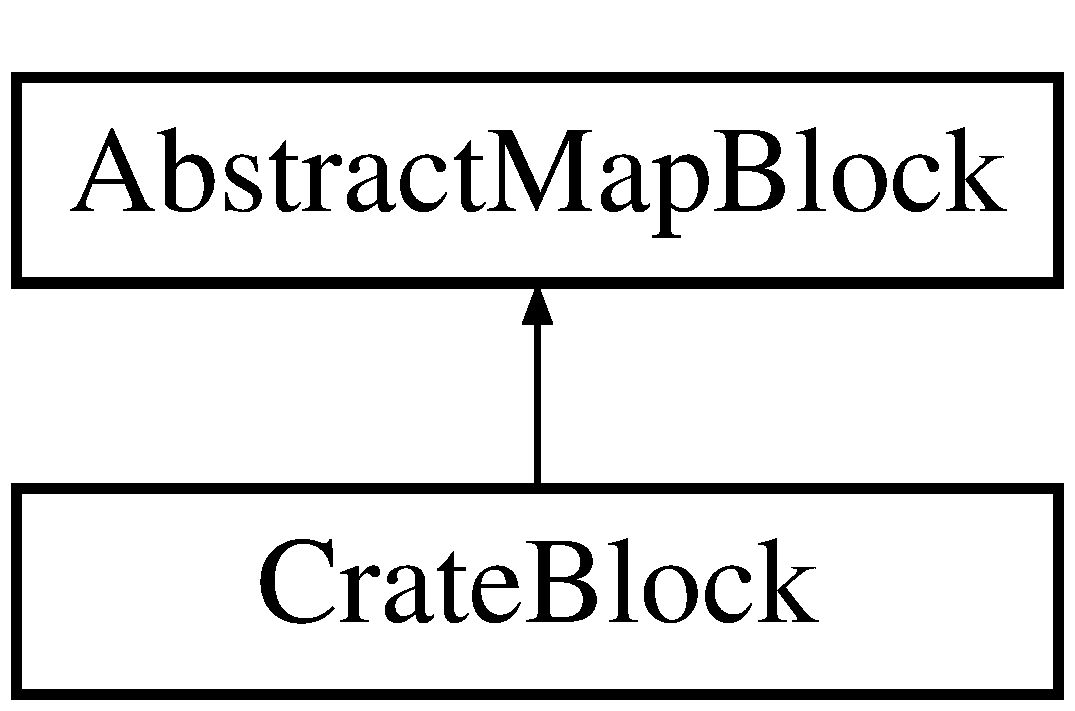
\includegraphics[height=2.000000cm]{class_crate_block}
\end{center}
\end{figure}
\subsection*{Public Member Functions}
\begin{DoxyCompactItemize}
\item 
\hyperlink{class_crate_block_a1a5d0818a3b1a878b7183b27461bcde4}{Crate\+Block} ()
\item 
\hyperlink{class_crate_block_af425285a43dc8a3eaf63a1abf91987cf}{Crate\+Block} (int x, int y)
\item 
\hyperlink{class_crate_block_aa853be5155fd0094454b2f25fb24c719}{$\sim$\+Crate\+Block} ()
\item 
sf\+::\+Sprite $\ast$ \hyperlink{class_crate_block_a1f478270194247d4e1f7f4b5eb883be9}{get\+Sprite} ()
\end{DoxyCompactItemize}
\subsection*{Protected Attributes}
\begin{DoxyCompactItemize}
\item 
sf\+::\+Texture $\ast$ \hyperlink{class_crate_block_a94ec4c6400389af2e8f1cd532c17eb5e}{texture}
\item 
sf\+::\+Sprite $\ast$ \hyperlink{class_crate_block_af4bed3d444d90dad4dd8a10c032c9724}{sprite}
\end{DoxyCompactItemize}
\subsection*{Additional Inherited Members}


\subsection{Detailed Description}
Blok reprezentujacy skrzynke w grze 

\subsection{Constructor \& Destructor Documentation}
\mbox{\Hypertarget{class_crate_block_a1a5d0818a3b1a878b7183b27461bcde4}\label{class_crate_block_a1a5d0818a3b1a878b7183b27461bcde4}} 
\index{Crate\+Block@{Crate\+Block}!Crate\+Block@{Crate\+Block}}
\index{Crate\+Block@{Crate\+Block}!Crate\+Block@{Crate\+Block}}
\subsubsection{\texorpdfstring{Crate\+Block()}{CrateBlock()}\hspace{0.1cm}{\footnotesize\ttfamily [1/2]}}
{\footnotesize\ttfamily Crate\+Block\+::\+Crate\+Block (\begin{DoxyParamCaption}{ }\end{DoxyParamCaption})}

Konstruktr bez parametrow, nie moze byc wywolywany! \mbox{\Hypertarget{class_crate_block_af425285a43dc8a3eaf63a1abf91987cf}\label{class_crate_block_af425285a43dc8a3eaf63a1abf91987cf}} 
\index{Crate\+Block@{Crate\+Block}!Crate\+Block@{Crate\+Block}}
\index{Crate\+Block@{Crate\+Block}!Crate\+Block@{Crate\+Block}}
\subsubsection{\texorpdfstring{Crate\+Block()}{CrateBlock()}\hspace{0.1cm}{\footnotesize\ttfamily [2/2]}}
{\footnotesize\ttfamily Crate\+Block\+::\+Crate\+Block (\begin{DoxyParamCaption}\item[{int}]{x,  }\item[{int}]{y }\end{DoxyParamCaption})}

Konstruktr, z parametrami x i y danego bloku, wzgledem mapy \mbox{\Hypertarget{class_crate_block_aa853be5155fd0094454b2f25fb24c719}\label{class_crate_block_aa853be5155fd0094454b2f25fb24c719}} 
\index{Crate\+Block@{Crate\+Block}!````~Crate\+Block@{$\sim$\+Crate\+Block}}
\index{````~Crate\+Block@{$\sim$\+Crate\+Block}!Crate\+Block@{Crate\+Block}}
\subsubsection{\texorpdfstring{$\sim$\+Crate\+Block()}{~CrateBlock()}}
{\footnotesize\ttfamily Crate\+Block\+::$\sim$\+Crate\+Block (\begin{DoxyParamCaption}{ }\end{DoxyParamCaption})}

Destruktor 

\subsection{Member Function Documentation}
\mbox{\Hypertarget{class_crate_block_a1f478270194247d4e1f7f4b5eb883be9}\label{class_crate_block_a1f478270194247d4e1f7f4b5eb883be9}} 
\index{Crate\+Block@{Crate\+Block}!get\+Sprite@{get\+Sprite}}
\index{get\+Sprite@{get\+Sprite}!Crate\+Block@{Crate\+Block}}
\subsubsection{\texorpdfstring{get\+Sprite()}{getSprite()}}
{\footnotesize\ttfamily sf\+::\+Sprite $\ast$ Crate\+Block\+::get\+Sprite (\begin{DoxyParamCaption}{ }\end{DoxyParamCaption})\hspace{0.3cm}{\ttfamily [virtual]}}

zwraca sprite-\/a 

Implements \hyperlink{class_abstract_map_block_ab5a448a1b6478d10a8814c6d19c4fdb4}{Abstract\+Map\+Block}.



\subsection{Member Data Documentation}
\mbox{\Hypertarget{class_crate_block_af4bed3d444d90dad4dd8a10c032c9724}\label{class_crate_block_af4bed3d444d90dad4dd8a10c032c9724}} 
\index{Crate\+Block@{Crate\+Block}!sprite@{sprite}}
\index{sprite@{sprite}!Crate\+Block@{Crate\+Block}}
\subsubsection{\texorpdfstring{sprite}{sprite}}
{\footnotesize\ttfamily sf\+::\+Sprite$\ast$ Crate\+Block\+::sprite\hspace{0.3cm}{\ttfamily [protected]}}

Sprite danego bloku \mbox{\Hypertarget{class_crate_block_a94ec4c6400389af2e8f1cd532c17eb5e}\label{class_crate_block_a94ec4c6400389af2e8f1cd532c17eb5e}} 
\index{Crate\+Block@{Crate\+Block}!texture@{texture}}
\index{texture@{texture}!Crate\+Block@{Crate\+Block}}
\subsubsection{\texorpdfstring{texture}{texture}}
{\footnotesize\ttfamily sf\+::\+Texture$\ast$ Crate\+Block\+::texture\hspace{0.3cm}{\ttfamily [protected]}}

Tekstura danego bloku 

The documentation for this class was generated from the following files\+:\begin{DoxyCompactItemize}
\item 
\hyperlink{_crate_block_8h}{Crate\+Block.\+h}\item 
\hyperlink{_crate_block_8cpp}{Crate\+Block.\+cpp}\end{DoxyCompactItemize}

\hypertarget{class_display_map_manager}{}\section{Display\+Map\+Manager Class Reference}
\label{class_display_map_manager}\index{Display\+Map\+Manager@{Display\+Map\+Manager}}


{\ttfamily \#include $<$Display\+Map\+Manager.\+h$>$}

\subsection*{Public Member Functions}
\begin{DoxyCompactItemize}
\item 
\hyperlink{class_display_map_manager_acca16727ef15d478af88df1acb8a1c89}{Display\+Map\+Manager} (\hyperlink{class_map}{Map} $\ast$\hyperlink{class_display_map_manager_aefa663d75781e47edfc5629e3652ead8}{map}, sf\+::\+Render\+Window $\ast$\hyperlink{class_display_map_manager_a880f01a1287f35cc4852c2e5d58ecd24}{window})
\item 
\hyperlink{class_display_map_manager_a9bce4856c4b749ce83a477d1801d1599}{$\sim$\+Display\+Map\+Manager} ()
\item 
void \hyperlink{class_display_map_manager_abd434e3d2795be7f9421f8bfe694d934}{display} (int x, int y)
\item 
void \hyperlink{class_display_map_manager_aff8cc85b9a149514ae95608ddbe20e10}{text\+Settings} ()
\item 
void \hyperlink{class_display_map_manager_a74e361f45d1e8366cbb1c0bba8ba7d0b}{animate\+Character} ()
\item 
void \hyperlink{class_display_map_manager_a9b8270c9ea4c4f5f036248719b4eae7c}{stop\+Animation} ()
\item 
bool \hyperlink{class_display_map_manager_af7e12870120f25befe945d54fe452288}{move\+Character\+Left} ()
\item 
bool \hyperlink{class_display_map_manager_ad17768ba9192593d2f0e6c8dad853899}{move\+Character\+Right} ()
\item 
bool \hyperlink{class_display_map_manager_ab1ed4f96b21f662039d3a96bafd75ca2}{move\+Character\+Up} ()
\item 
bool \hyperlink{class_display_map_manager_a9d19cecb4e669680321fef6d3e85910c}{move\+Character\+Down} ()
\end{DoxyCompactItemize}
\subsection*{Public Attributes}
\begin{DoxyCompactItemize}
\item 
\hyperlink{class_map}{Map} $\ast$ \hyperlink{class_display_map_manager_aefa663d75781e47edfc5629e3652ead8}{map}
\item 
sf\+::\+Render\+Window $\ast$ \hyperlink{class_display_map_manager_a880f01a1287f35cc4852c2e5d58ecd24}{window}
\item 
sf\+::\+Clock \hyperlink{class_display_map_manager_ad04d2e96cd8ba8f1cbcf3425bd28cfc5}{clock}
\item 
sf\+::\+Font \hyperlink{class_display_map_manager_af1ea34885ea77010e9a99b6a49da5e58}{My\+Font}
\item 
sf\+::\+Text \hyperlink{class_display_map_manager_ad9a89d13fbf1ac95fbb058b565bb4d2f}{text}
\end{DoxyCompactItemize}
\subsection*{Protected Member Functions}
\begin{DoxyCompactItemize}
\item 
float \hyperlink{class_display_map_manager_a9f3a6841688b7e4932ca1269588d4504}{get\+Character\+WindowX} ()
\item 
float \hyperlink{class_display_map_manager_a4a17bf69eb158d10c6af0b5467735d60}{get\+Character\+WindowY} ()
\item 
float \hyperlink{class_display_map_manager_af26ef96ab1e1e2c33e9160a8a66263f7}{get\+Window\+X\+Postion} (float map\+X\+Postion)
\item 
float \hyperlink{class_display_map_manager_ad850ee0bd93bab3cf376ce343eabfff0}{get\+Window\+Y\+Postion} (float map\+Y\+Postion)
\item 
float \hyperlink{class_display_map_manager_a12847fea83dc76f47255605f7de3d020}{get\+Background\+Window\+X\+Position} (float character\+Position\+MapX)
\item 
float \hyperlink{class_display_map_manager_a7326948a0f1ef16c89a27f5bde09192b}{get\+Background\+Window\+Y\+Position} (float character\+Position\+MapY)
\end{DoxyCompactItemize}


\subsection{Constructor \& Destructor Documentation}
\mbox{\Hypertarget{class_display_map_manager_acca16727ef15d478af88df1acb8a1c89}\label{class_display_map_manager_acca16727ef15d478af88df1acb8a1c89}} 
\index{Display\+Map\+Manager@{Display\+Map\+Manager}!Display\+Map\+Manager@{Display\+Map\+Manager}}
\index{Display\+Map\+Manager@{Display\+Map\+Manager}!Display\+Map\+Manager@{Display\+Map\+Manager}}
\subsubsection{\texorpdfstring{Display\+Map\+Manager()}{DisplayMapManager()}}
{\footnotesize\ttfamily Display\+Map\+Manager\+::\+Display\+Map\+Manager (\begin{DoxyParamCaption}\item[{\hyperlink{class_map}{Map} $\ast$}]{map,  }\item[{sf\+::\+Render\+Window $\ast$}]{window }\end{DoxyParamCaption})}

\mbox{\Hypertarget{class_display_map_manager_a9bce4856c4b749ce83a477d1801d1599}\label{class_display_map_manager_a9bce4856c4b749ce83a477d1801d1599}} 
\index{Display\+Map\+Manager@{Display\+Map\+Manager}!````~Display\+Map\+Manager@{$\sim$\+Display\+Map\+Manager}}
\index{````~Display\+Map\+Manager@{$\sim$\+Display\+Map\+Manager}!Display\+Map\+Manager@{Display\+Map\+Manager}}
\subsubsection{\texorpdfstring{$\sim$\+Display\+Map\+Manager()}{~DisplayMapManager()}}
{\footnotesize\ttfamily Display\+Map\+Manager\+::$\sim$\+Display\+Map\+Manager (\begin{DoxyParamCaption}{ }\end{DoxyParamCaption})}



\subsection{Member Function Documentation}
\mbox{\Hypertarget{class_display_map_manager_a74e361f45d1e8366cbb1c0bba8ba7d0b}\label{class_display_map_manager_a74e361f45d1e8366cbb1c0bba8ba7d0b}} 
\index{Display\+Map\+Manager@{Display\+Map\+Manager}!animate\+Character@{animate\+Character}}
\index{animate\+Character@{animate\+Character}!Display\+Map\+Manager@{Display\+Map\+Manager}}
\subsubsection{\texorpdfstring{animate\+Character()}{animateCharacter()}}
{\footnotesize\ttfamily void Display\+Map\+Manager\+::animate\+Character (\begin{DoxyParamCaption}{ }\end{DoxyParamCaption})}

\mbox{\Hypertarget{class_display_map_manager_abd434e3d2795be7f9421f8bfe694d934}\label{class_display_map_manager_abd434e3d2795be7f9421f8bfe694d934}} 
\index{Display\+Map\+Manager@{Display\+Map\+Manager}!display@{display}}
\index{display@{display}!Display\+Map\+Manager@{Display\+Map\+Manager}}
\subsubsection{\texorpdfstring{display()}{display()}}
{\footnotesize\ttfamily void Display\+Map\+Manager\+::display (\begin{DoxyParamCaption}\item[{int}]{x,  }\item[{int}]{y }\end{DoxyParamCaption})}

\mbox{\Hypertarget{class_display_map_manager_a12847fea83dc76f47255605f7de3d020}\label{class_display_map_manager_a12847fea83dc76f47255605f7de3d020}} 
\index{Display\+Map\+Manager@{Display\+Map\+Manager}!get\+Background\+Window\+X\+Position@{get\+Background\+Window\+X\+Position}}
\index{get\+Background\+Window\+X\+Position@{get\+Background\+Window\+X\+Position}!Display\+Map\+Manager@{Display\+Map\+Manager}}
\subsubsection{\texorpdfstring{get\+Background\+Window\+X\+Position()}{getBackgroundWindowXPosition()}}
{\footnotesize\ttfamily float Display\+Map\+Manager\+::get\+Background\+Window\+X\+Position (\begin{DoxyParamCaption}\item[{float}]{character\+Position\+MapX }\end{DoxyParamCaption})\hspace{0.3cm}{\ttfamily [protected]}}

\mbox{\Hypertarget{class_display_map_manager_a7326948a0f1ef16c89a27f5bde09192b}\label{class_display_map_manager_a7326948a0f1ef16c89a27f5bde09192b}} 
\index{Display\+Map\+Manager@{Display\+Map\+Manager}!get\+Background\+Window\+Y\+Position@{get\+Background\+Window\+Y\+Position}}
\index{get\+Background\+Window\+Y\+Position@{get\+Background\+Window\+Y\+Position}!Display\+Map\+Manager@{Display\+Map\+Manager}}
\subsubsection{\texorpdfstring{get\+Background\+Window\+Y\+Position()}{getBackgroundWindowYPosition()}}
{\footnotesize\ttfamily float Display\+Map\+Manager\+::get\+Background\+Window\+Y\+Position (\begin{DoxyParamCaption}\item[{float}]{character\+Position\+MapY }\end{DoxyParamCaption})\hspace{0.3cm}{\ttfamily [protected]}}

\mbox{\Hypertarget{class_display_map_manager_a9f3a6841688b7e4932ca1269588d4504}\label{class_display_map_manager_a9f3a6841688b7e4932ca1269588d4504}} 
\index{Display\+Map\+Manager@{Display\+Map\+Manager}!get\+Character\+WindowX@{get\+Character\+WindowX}}
\index{get\+Character\+WindowX@{get\+Character\+WindowX}!Display\+Map\+Manager@{Display\+Map\+Manager}}
\subsubsection{\texorpdfstring{get\+Character\+Window\+X()}{getCharacterWindowX()}}
{\footnotesize\ttfamily float Display\+Map\+Manager\+::get\+Character\+WindowX (\begin{DoxyParamCaption}{ }\end{DoxyParamCaption})\hspace{0.3cm}{\ttfamily [protected]}}

\mbox{\Hypertarget{class_display_map_manager_a4a17bf69eb158d10c6af0b5467735d60}\label{class_display_map_manager_a4a17bf69eb158d10c6af0b5467735d60}} 
\index{Display\+Map\+Manager@{Display\+Map\+Manager}!get\+Character\+WindowY@{get\+Character\+WindowY}}
\index{get\+Character\+WindowY@{get\+Character\+WindowY}!Display\+Map\+Manager@{Display\+Map\+Manager}}
\subsubsection{\texorpdfstring{get\+Character\+Window\+Y()}{getCharacterWindowY()}}
{\footnotesize\ttfamily float Display\+Map\+Manager\+::get\+Character\+WindowY (\begin{DoxyParamCaption}{ }\end{DoxyParamCaption})\hspace{0.3cm}{\ttfamily [protected]}}

\mbox{\Hypertarget{class_display_map_manager_af26ef96ab1e1e2c33e9160a8a66263f7}\label{class_display_map_manager_af26ef96ab1e1e2c33e9160a8a66263f7}} 
\index{Display\+Map\+Manager@{Display\+Map\+Manager}!get\+Window\+X\+Postion@{get\+Window\+X\+Postion}}
\index{get\+Window\+X\+Postion@{get\+Window\+X\+Postion}!Display\+Map\+Manager@{Display\+Map\+Manager}}
\subsubsection{\texorpdfstring{get\+Window\+X\+Postion()}{getWindowXPostion()}}
{\footnotesize\ttfamily float Display\+Map\+Manager\+::get\+Window\+X\+Postion (\begin{DoxyParamCaption}\item[{float}]{map\+X\+Postion }\end{DoxyParamCaption})\hspace{0.3cm}{\ttfamily [protected]}}

\mbox{\Hypertarget{class_display_map_manager_ad850ee0bd93bab3cf376ce343eabfff0}\label{class_display_map_manager_ad850ee0bd93bab3cf376ce343eabfff0}} 
\index{Display\+Map\+Manager@{Display\+Map\+Manager}!get\+Window\+Y\+Postion@{get\+Window\+Y\+Postion}}
\index{get\+Window\+Y\+Postion@{get\+Window\+Y\+Postion}!Display\+Map\+Manager@{Display\+Map\+Manager}}
\subsubsection{\texorpdfstring{get\+Window\+Y\+Postion()}{getWindowYPostion()}}
{\footnotesize\ttfamily float Display\+Map\+Manager\+::get\+Window\+Y\+Postion (\begin{DoxyParamCaption}\item[{float}]{map\+Y\+Postion }\end{DoxyParamCaption})\hspace{0.3cm}{\ttfamily [protected]}}

\mbox{\Hypertarget{class_display_map_manager_a9d19cecb4e669680321fef6d3e85910c}\label{class_display_map_manager_a9d19cecb4e669680321fef6d3e85910c}} 
\index{Display\+Map\+Manager@{Display\+Map\+Manager}!move\+Character\+Down@{move\+Character\+Down}}
\index{move\+Character\+Down@{move\+Character\+Down}!Display\+Map\+Manager@{Display\+Map\+Manager}}
\subsubsection{\texorpdfstring{move\+Character\+Down()}{moveCharacterDown()}}
{\footnotesize\ttfamily bool Display\+Map\+Manager\+::move\+Character\+Down (\begin{DoxyParamCaption}{ }\end{DoxyParamCaption})}

\mbox{\Hypertarget{class_display_map_manager_af7e12870120f25befe945d54fe452288}\label{class_display_map_manager_af7e12870120f25befe945d54fe452288}} 
\index{Display\+Map\+Manager@{Display\+Map\+Manager}!move\+Character\+Left@{move\+Character\+Left}}
\index{move\+Character\+Left@{move\+Character\+Left}!Display\+Map\+Manager@{Display\+Map\+Manager}}
\subsubsection{\texorpdfstring{move\+Character\+Left()}{moveCharacterLeft()}}
{\footnotesize\ttfamily bool Display\+Map\+Manager\+::move\+Character\+Left (\begin{DoxyParamCaption}{ }\end{DoxyParamCaption})}

\mbox{\Hypertarget{class_display_map_manager_ad17768ba9192593d2f0e6c8dad853899}\label{class_display_map_manager_ad17768ba9192593d2f0e6c8dad853899}} 
\index{Display\+Map\+Manager@{Display\+Map\+Manager}!move\+Character\+Right@{move\+Character\+Right}}
\index{move\+Character\+Right@{move\+Character\+Right}!Display\+Map\+Manager@{Display\+Map\+Manager}}
\subsubsection{\texorpdfstring{move\+Character\+Right()}{moveCharacterRight()}}
{\footnotesize\ttfamily bool Display\+Map\+Manager\+::move\+Character\+Right (\begin{DoxyParamCaption}{ }\end{DoxyParamCaption})}

\mbox{\Hypertarget{class_display_map_manager_ab1ed4f96b21f662039d3a96bafd75ca2}\label{class_display_map_manager_ab1ed4f96b21f662039d3a96bafd75ca2}} 
\index{Display\+Map\+Manager@{Display\+Map\+Manager}!move\+Character\+Up@{move\+Character\+Up}}
\index{move\+Character\+Up@{move\+Character\+Up}!Display\+Map\+Manager@{Display\+Map\+Manager}}
\subsubsection{\texorpdfstring{move\+Character\+Up()}{moveCharacterUp()}}
{\footnotesize\ttfamily bool Display\+Map\+Manager\+::move\+Character\+Up (\begin{DoxyParamCaption}{ }\end{DoxyParamCaption})}

\mbox{\Hypertarget{class_display_map_manager_a9b8270c9ea4c4f5f036248719b4eae7c}\label{class_display_map_manager_a9b8270c9ea4c4f5f036248719b4eae7c}} 
\index{Display\+Map\+Manager@{Display\+Map\+Manager}!stop\+Animation@{stop\+Animation}}
\index{stop\+Animation@{stop\+Animation}!Display\+Map\+Manager@{Display\+Map\+Manager}}
\subsubsection{\texorpdfstring{stop\+Animation()}{stopAnimation()}}
{\footnotesize\ttfamily void Display\+Map\+Manager\+::stop\+Animation (\begin{DoxyParamCaption}{ }\end{DoxyParamCaption})}

\mbox{\Hypertarget{class_display_map_manager_aff8cc85b9a149514ae95608ddbe20e10}\label{class_display_map_manager_aff8cc85b9a149514ae95608ddbe20e10}} 
\index{Display\+Map\+Manager@{Display\+Map\+Manager}!text\+Settings@{text\+Settings}}
\index{text\+Settings@{text\+Settings}!Display\+Map\+Manager@{Display\+Map\+Manager}}
\subsubsection{\texorpdfstring{text\+Settings()}{textSettings()}}
{\footnotesize\ttfamily void Display\+Map\+Manager\+::text\+Settings (\begin{DoxyParamCaption}{ }\end{DoxyParamCaption})}



\subsection{Member Data Documentation}
\mbox{\Hypertarget{class_display_map_manager_ad04d2e96cd8ba8f1cbcf3425bd28cfc5}\label{class_display_map_manager_ad04d2e96cd8ba8f1cbcf3425bd28cfc5}} 
\index{Display\+Map\+Manager@{Display\+Map\+Manager}!clock@{clock}}
\index{clock@{clock}!Display\+Map\+Manager@{Display\+Map\+Manager}}
\subsubsection{\texorpdfstring{clock}{clock}}
{\footnotesize\ttfamily sf\+::\+Clock Display\+Map\+Manager\+::clock}

\mbox{\Hypertarget{class_display_map_manager_aefa663d75781e47edfc5629e3652ead8}\label{class_display_map_manager_aefa663d75781e47edfc5629e3652ead8}} 
\index{Display\+Map\+Manager@{Display\+Map\+Manager}!map@{map}}
\index{map@{map}!Display\+Map\+Manager@{Display\+Map\+Manager}}
\subsubsection{\texorpdfstring{map}{map}}
{\footnotesize\ttfamily \hyperlink{class_map}{Map}$\ast$ Display\+Map\+Manager\+::map}

\mbox{\Hypertarget{class_display_map_manager_af1ea34885ea77010e9a99b6a49da5e58}\label{class_display_map_manager_af1ea34885ea77010e9a99b6a49da5e58}} 
\index{Display\+Map\+Manager@{Display\+Map\+Manager}!My\+Font@{My\+Font}}
\index{My\+Font@{My\+Font}!Display\+Map\+Manager@{Display\+Map\+Manager}}
\subsubsection{\texorpdfstring{My\+Font}{MyFont}}
{\footnotesize\ttfamily sf\+::\+Font Display\+Map\+Manager\+::\+My\+Font}

\mbox{\Hypertarget{class_display_map_manager_ad9a89d13fbf1ac95fbb058b565bb4d2f}\label{class_display_map_manager_ad9a89d13fbf1ac95fbb058b565bb4d2f}} 
\index{Display\+Map\+Manager@{Display\+Map\+Manager}!text@{text}}
\index{text@{text}!Display\+Map\+Manager@{Display\+Map\+Manager}}
\subsubsection{\texorpdfstring{text}{text}}
{\footnotesize\ttfamily sf\+::\+Text Display\+Map\+Manager\+::text}

\mbox{\Hypertarget{class_display_map_manager_a880f01a1287f35cc4852c2e5d58ecd24}\label{class_display_map_manager_a880f01a1287f35cc4852c2e5d58ecd24}} 
\index{Display\+Map\+Manager@{Display\+Map\+Manager}!window@{window}}
\index{window@{window}!Display\+Map\+Manager@{Display\+Map\+Manager}}
\subsubsection{\texorpdfstring{window}{window}}
{\footnotesize\ttfamily sf\+::\+Render\+Window$\ast$ Display\+Map\+Manager\+::window}



The documentation for this class was generated from the following files\+:\begin{DoxyCompactItemize}
\item 
\hyperlink{_display_map_manager_8h}{Display\+Map\+Manager.\+h}\item 
\hyperlink{_display_map_manager_8cpp}{Display\+Map\+Manager.\+cpp}\end{DoxyCompactItemize}

\hypertarget{class_gravity}{}\section{Gravity Class Reference}
\label{class_gravity}\index{Gravity@{Gravity}}
\subsection*{Public Member Functions}
\begin{DoxyCompactItemize}
\item 
\mbox{\Hypertarget{class_gravity_a366c547f2ab1425b5e6981b15a55852d}\label{class_gravity_a366c547f2ab1425b5e6981b15a55852d}} 
{\bfseries Gravity} (\hyperlink{class_display_map_manager}{Display\+Map\+Manager} $\ast$display\+Map\+Manager)
\item 
\mbox{\Hypertarget{class_gravity_a350121b3d211c4740f3715acc64987e3}\label{class_gravity_a350121b3d211c4740f3715acc64987e3}} 
void {\bfseries interact\+Gravity} ()
\item 
\mbox{\Hypertarget{class_gravity_adb2abc628833f3424ad3ddb93e581290}\label{class_gravity_adb2abc628833f3424ad3ddb93e581290}} 
void {\bfseries character\+Jump} ()
\item 
\mbox{\Hypertarget{class_gravity_a827989f236cfa0cb2732869f352b4057}\label{class_gravity_a827989f236cfa0cb2732869f352b4057}} 
void {\bfseries stop\+Jump} ()
\end{DoxyCompactItemize}
\subsection*{Public Attributes}
\begin{DoxyCompactItemize}
\item 
\mbox{\Hypertarget{class_gravity_a3a942e2b771c8a764914cb18c8bef394}\label{class_gravity_a3a942e2b771c8a764914cb18c8bef394}} 
sf\+::\+Sound\+Buffer {\bfseries buffer}
\item 
\mbox{\Hypertarget{class_gravity_a5d636ab38b930cff4d585bfd374479b6}\label{class_gravity_a5d636ab38b930cff4d585bfd374479b6}} 
sf\+::\+Sound {\bfseries sound}
\end{DoxyCompactItemize}
\subsection*{Protected Attributes}
\begin{DoxyCompactItemize}
\item 
\mbox{\Hypertarget{class_gravity_a72a7e04f7555e0f29d100c965ff5080f}\label{class_gravity_a72a7e04f7555e0f29d100c965ff5080f}} 
\hyperlink{class_display_map_manager}{Display\+Map\+Manager} $\ast$ {\bfseries display\+Map\+Manager}
\item 
\mbox{\Hypertarget{class_gravity_a9284458ed2208a9df9ea8f1bf1b6c36a}\label{class_gravity_a9284458ed2208a9df9ea8f1bf1b6c36a}} 
sf\+::\+Time {\bfseries start\+Jump}
\item 
\mbox{\Hypertarget{class_gravity_ac126e399cf8cc40a6267b8f099865042}\label{class_gravity_ac126e399cf8cc40a6267b8f099865042}} 
sf\+::\+Clock {\bfseries clock}
\end{DoxyCompactItemize}


The documentation for this class was generated from the following files\+:\begin{DoxyCompactItemize}
\item 
Gravity.\+h\item 
Gravity.\+cpp\end{DoxyCompactItemize}

\hypertarget{class_ground_block}{}\section{Ground\+Block Class Reference}
\label{class_ground_block}\index{Ground\+Block@{Ground\+Block}}
Inheritance diagram for Ground\+Block\+:\begin{figure}[H]
\begin{center}
\leavevmode
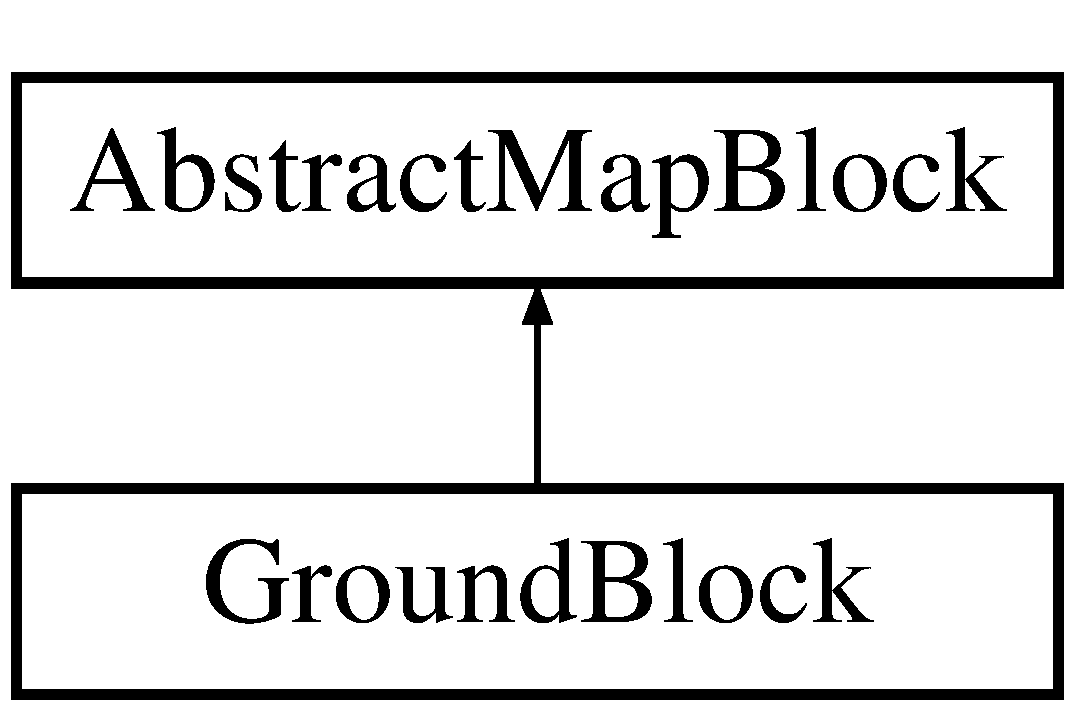
\includegraphics[height=2.000000cm]{class_ground_block}
\end{center}
\end{figure}
\subsection*{Public Member Functions}
\begin{DoxyCompactItemize}
\item 
\mbox{\Hypertarget{class_ground_block_a0155a6938214c2752002828b9e26da0a}\label{class_ground_block_a0155a6938214c2752002828b9e26da0a}} 
{\bfseries Ground\+Block} (int x, int y)
\item 
\mbox{\Hypertarget{class_ground_block_a73c0f8ff59ef53b18f03bc3f22f8f810}\label{class_ground_block_a73c0f8ff59ef53b18f03bc3f22f8f810}} 
sf\+::\+Sprite $\ast$ {\bfseries get\+Sprite} ()
\end{DoxyCompactItemize}
\subsection*{Protected Attributes}
\begin{DoxyCompactItemize}
\item 
\mbox{\Hypertarget{class_ground_block_af610cda7ad96e934524a7bbdc13a64d6}\label{class_ground_block_af610cda7ad96e934524a7bbdc13a64d6}} 
sf\+::\+Texture $\ast$ {\bfseries texture}
\item 
\mbox{\Hypertarget{class_ground_block_a235135fde9ffb53700b4bee134175dda}\label{class_ground_block_a235135fde9ffb53700b4bee134175dda}} 
sf\+::\+Sprite $\ast$ {\bfseries sprite}
\end{DoxyCompactItemize}
\subsection*{Additional Inherited Members}


The documentation for this class was generated from the following files\+:\begin{DoxyCompactItemize}
\item 
Ground\+Block.\+h\item 
Ground\+Block.\+cpp\end{DoxyCompactItemize}

\hypertarget{class_map}{}\section{Map Class Reference}
\label{class_map}\index{Map@{Map}}


{\ttfamily \#include $<$Map.\+h$>$}

\subsection*{Public Member Functions}
\begin{DoxyCompactItemize}
\item 
\hyperlink{class_map_a0f5ad0fd4563497b4214038cbca8b582}{Map} ()
\item 
\hyperlink{class_map_aa403fbe09394ccf39747588f5168e3b2}{$\sim$\+Map} ()
\item 
bool \hyperlink{class_map_a9e0db2b7f0c2cc2083da543050f0fa91}{can\+Move} (float x, float y)
\item 
int \hyperlink{class_map_a46c8ba4683ce97e3f5120be02b0ace94}{get\+X\+Elem\+Pos} (int col)
\item 
int \hyperlink{class_map_a8efab6f1e807cb4cb576fc5dcfed3075}{get\+Y\+Elem\+Pos} (int row)
\end{DoxyCompactItemize}
\subsection*{Public Attributes}
\begin{DoxyCompactItemize}
\item 
\hyperlink{class_character}{Character} \hyperlink{class_map_a00d7fac6e87f2ac95d0182bbb22fdac4}{character}
\item 
sf\+::\+Texture \hyperlink{class_map_a18202f9ebc5ddab14652bdacc81e3c72}{background\+Texture}
\item 
sf\+::\+Sprite \hyperlink{class_map_aa92b0ecd899641e3385613efcd037f65}{background\+Sprite}
\item 
int \hyperlink{class_map_ac62ec077cb012a9fe7d987b466a48947}{width\+Map}
\item 
float \hyperlink{class_map_acfd2fda55638ba32a092fac314f9f1c5}{character\+Position\+MapX}
\item 
float \hyperlink{class_map_aa4e4d68c7babc74782b973a3b97431ea}{character\+Position\+MapY}
\item 
std\+::list$<$ \hyperlink{class_abstract_map_block}{Abstract\+Map\+Block} $\ast$ $>$ \hyperlink{class_map_ad185fe5369037999533e218f3f7ade8a}{block\+List}
\end{DoxyCompactItemize}


\subsection{Detailed Description}
Reprezentacja mapy w grze. Przechowuje wszyskie bloki jakie istniejan na mapie 

\subsection{Constructor \& Destructor Documentation}
\mbox{\Hypertarget{class_map_a0f5ad0fd4563497b4214038cbca8b582}\label{class_map_a0f5ad0fd4563497b4214038cbca8b582}} 
\index{Map@{Map}!Map@{Map}}
\index{Map@{Map}!Map@{Map}}
\subsubsection{\texorpdfstring{Map()}{Map()}}
{\footnotesize\ttfamily Map\+::\+Map (\begin{DoxyParamCaption}{ }\end{DoxyParamCaption})}

konstruktor \mbox{\Hypertarget{class_map_aa403fbe09394ccf39747588f5168e3b2}\label{class_map_aa403fbe09394ccf39747588f5168e3b2}} 
\index{Map@{Map}!````~Map@{$\sim$\+Map}}
\index{````~Map@{$\sim$\+Map}!Map@{Map}}
\subsubsection{\texorpdfstring{$\sim$\+Map()}{~Map()}}
{\footnotesize\ttfamily Map\+::$\sim$\+Map (\begin{DoxyParamCaption}{ }\end{DoxyParamCaption})}

destruktor 

\subsection{Member Function Documentation}
\mbox{\Hypertarget{class_map_a9e0db2b7f0c2cc2083da543050f0fa91}\label{class_map_a9e0db2b7f0c2cc2083da543050f0fa91}} 
\index{Map@{Map}!can\+Move@{can\+Move}}
\index{can\+Move@{can\+Move}!Map@{Map}}
\subsubsection{\texorpdfstring{can\+Move()}{canMove()}}
{\footnotesize\ttfamily bool Map\+::can\+Move (\begin{DoxyParamCaption}\item[{float}]{x,  }\item[{float}]{y }\end{DoxyParamCaption})}

sprawdza czy gracz moze sie przesunac do danej wsp mapy. Jesli dla danej wsp istnieje blok na mapie, zwraca false \mbox{\Hypertarget{class_map_a46c8ba4683ce97e3f5120be02b0ace94}\label{class_map_a46c8ba4683ce97e3f5120be02b0ace94}} 
\index{Map@{Map}!get\+X\+Elem\+Pos@{get\+X\+Elem\+Pos}}
\index{get\+X\+Elem\+Pos@{get\+X\+Elem\+Pos}!Map@{Map}}
\subsubsection{\texorpdfstring{get\+X\+Elem\+Pos()}{getXElemPos()}}
{\footnotesize\ttfamily int Map\+::get\+X\+Elem\+Pos (\begin{DoxyParamCaption}\item[{int}]{col }\end{DoxyParamCaption})}

mapa podzielona jest na kolumny. Zwraca wsp x dla danej kolumny \mbox{\Hypertarget{class_map_a8efab6f1e807cb4cb576fc5dcfed3075}\label{class_map_a8efab6f1e807cb4cb576fc5dcfed3075}} 
\index{Map@{Map}!get\+Y\+Elem\+Pos@{get\+Y\+Elem\+Pos}}
\index{get\+Y\+Elem\+Pos@{get\+Y\+Elem\+Pos}!Map@{Map}}
\subsubsection{\texorpdfstring{get\+Y\+Elem\+Pos()}{getYElemPos()}}
{\footnotesize\ttfamily int Map\+::get\+Y\+Elem\+Pos (\begin{DoxyParamCaption}\item[{int}]{row }\end{DoxyParamCaption})}

mapa podzielona jest na wiersze. Zwraca wsp y danego wiersza 

\subsection{Member Data Documentation}
\mbox{\Hypertarget{class_map_aa92b0ecd899641e3385613efcd037f65}\label{class_map_aa92b0ecd899641e3385613efcd037f65}} 
\index{Map@{Map}!background\+Sprite@{background\+Sprite}}
\index{background\+Sprite@{background\+Sprite}!Map@{Map}}
\subsubsection{\texorpdfstring{background\+Sprite}{backgroundSprite}}
{\footnotesize\ttfamily sf\+::\+Sprite Map\+::background\+Sprite}

sprite tla mapy \mbox{\Hypertarget{class_map_a18202f9ebc5ddab14652bdacc81e3c72}\label{class_map_a18202f9ebc5ddab14652bdacc81e3c72}} 
\index{Map@{Map}!background\+Texture@{background\+Texture}}
\index{background\+Texture@{background\+Texture}!Map@{Map}}
\subsubsection{\texorpdfstring{background\+Texture}{backgroundTexture}}
{\footnotesize\ttfamily sf\+::\+Texture Map\+::background\+Texture}

tekstura tla mapy \mbox{\Hypertarget{class_map_ad185fe5369037999533e218f3f7ade8a}\label{class_map_ad185fe5369037999533e218f3f7ade8a}} 
\index{Map@{Map}!block\+List@{block\+List}}
\index{block\+List@{block\+List}!Map@{Map}}
\subsubsection{\texorpdfstring{block\+List}{blockList}}
{\footnotesize\ttfamily std\+::list$<$\hyperlink{class_abstract_map_block}{Abstract\+Map\+Block} $\ast$$>$ Map\+::block\+List}

lista wszystkich blokow uzywanych w mapie \mbox{\Hypertarget{class_map_a00d7fac6e87f2ac95d0182bbb22fdac4}\label{class_map_a00d7fac6e87f2ac95d0182bbb22fdac4}} 
\index{Map@{Map}!character@{character}}
\index{character@{character}!Map@{Map}}
\subsubsection{\texorpdfstring{character}{character}}
{\footnotesize\ttfamily \hyperlink{class_character}{Character} Map\+::character}

Reprezentacja postaci w grze \mbox{\Hypertarget{class_map_acfd2fda55638ba32a092fac314f9f1c5}\label{class_map_acfd2fda55638ba32a092fac314f9f1c5}} 
\index{Map@{Map}!character\+Position\+MapX@{character\+Position\+MapX}}
\index{character\+Position\+MapX@{character\+Position\+MapX}!Map@{Map}}
\subsubsection{\texorpdfstring{character\+Position\+MapX}{characterPositionMapX}}
{\footnotesize\ttfamily float Map\+::character\+Position\+MapX}

pozycja x gracza na mapie (zgledem lewego gornego rogu mapy) \mbox{\Hypertarget{class_map_aa4e4d68c7babc74782b973a3b97431ea}\label{class_map_aa4e4d68c7babc74782b973a3b97431ea}} 
\index{Map@{Map}!character\+Position\+MapY@{character\+Position\+MapY}}
\index{character\+Position\+MapY@{character\+Position\+MapY}!Map@{Map}}
\subsubsection{\texorpdfstring{character\+Position\+MapY}{characterPositionMapY}}
{\footnotesize\ttfamily float Map\+::character\+Position\+MapY}

pozycja y gracza na mapie (zgledem lewego gornego rogu mapy) \mbox{\Hypertarget{class_map_ac62ec077cb012a9fe7d987b466a48947}\label{class_map_ac62ec077cb012a9fe7d987b466a48947}} 
\index{Map@{Map}!width\+Map@{width\+Map}}
\index{width\+Map@{width\+Map}!Map@{Map}}
\subsubsection{\texorpdfstring{width\+Map}{widthMap}}
{\footnotesize\ttfamily int Map\+::width\+Map}

szerokosc mapy 

The documentation for this class was generated from the following files\+:\begin{DoxyCompactItemize}
\item 
\hyperlink{_map_8h}{Map.\+h}\item 
\hyperlink{_map_8cpp}{Map.\+cpp}\end{DoxyCompactItemize}

\hypertarget{class_plank_block}{}\section{Plank\+Block Class Reference}
\label{class_plank_block}\index{Plank\+Block@{Plank\+Block}}


{\ttfamily \#include $<$Plank\+Block.\+h$>$}

Inheritance diagram for Plank\+Block\+:\begin{figure}[H]
\begin{center}
\leavevmode
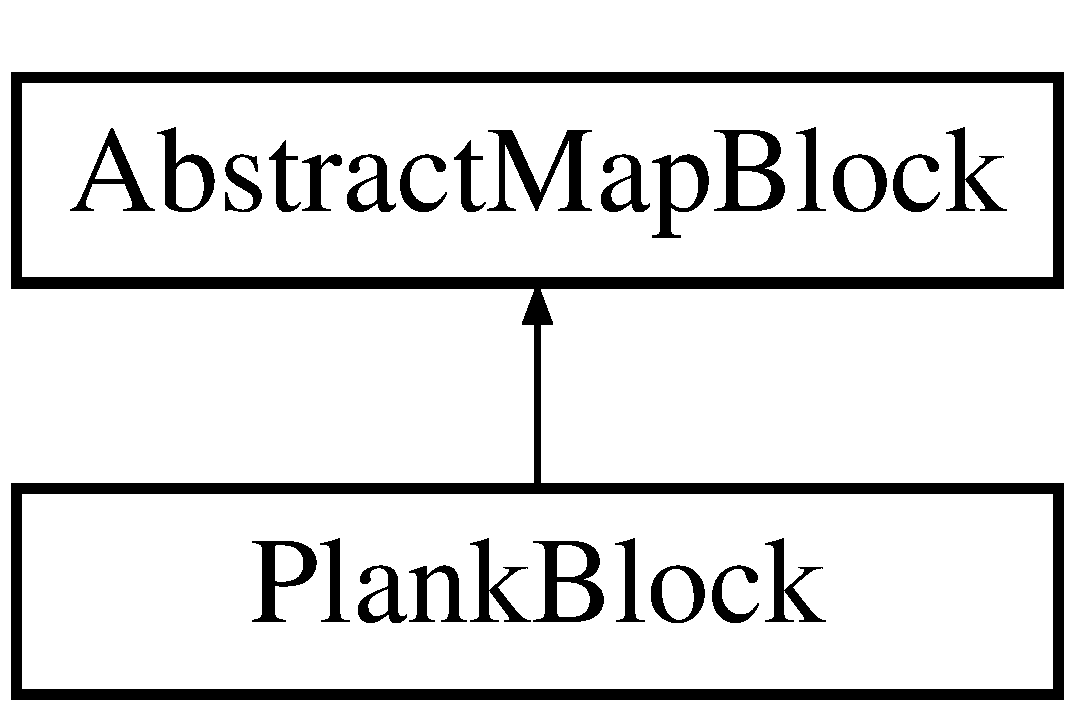
\includegraphics[height=2.000000cm]{class_plank_block}
\end{center}
\end{figure}
\subsection*{Public Member Functions}
\begin{DoxyCompactItemize}
\item 
\hyperlink{class_plank_block_af0a7e46056468e24b74c0aca475533b9}{Plank\+Block} ()
\item 
\hyperlink{class_plank_block_afed7c0965c7e1e4b9ec98a4ff06825df}{Plank\+Block} (int x, int y)
\item 
\hyperlink{class_plank_block_afbd822caf201cd34777e46addb7f50c8}{$\sim$\+Plank\+Block} ()
\item 
sf\+::\+Sprite $\ast$ \hyperlink{class_plank_block_abada589bb200fd82fcfe00482ad6a32f}{get\+Sprite} ()
\end{DoxyCompactItemize}
\subsection*{Protected Attributes}
\begin{DoxyCompactItemize}
\item 
sf\+::\+Texture $\ast$ \hyperlink{class_plank_block_a9b6bada075fecb031e3db24eff50fd19}{texture}
\item 
sf\+::\+Sprite $\ast$ \hyperlink{class_plank_block_a28e42e2ccc8973b39b3c1fbdeee78c36}{sprite}
\end{DoxyCompactItemize}
\subsection*{Additional Inherited Members}


\subsection{Detailed Description}
Blok reprezentujacy drewniana platforme w grze 

\subsection{Constructor \& Destructor Documentation}
\mbox{\Hypertarget{class_plank_block_af0a7e46056468e24b74c0aca475533b9}\label{class_plank_block_af0a7e46056468e24b74c0aca475533b9}} 
\index{Plank\+Block@{Plank\+Block}!Plank\+Block@{Plank\+Block}}
\index{Plank\+Block@{Plank\+Block}!Plank\+Block@{Plank\+Block}}
\subsubsection{\texorpdfstring{Plank\+Block()}{PlankBlock()}\hspace{0.1cm}{\footnotesize\ttfamily [1/2]}}
{\footnotesize\ttfamily Plank\+Block\+::\+Plank\+Block (\begin{DoxyParamCaption}{ }\end{DoxyParamCaption})}

Konstruktr bez parametrow, nie moze byc wywolywany! \mbox{\Hypertarget{class_plank_block_afed7c0965c7e1e4b9ec98a4ff06825df}\label{class_plank_block_afed7c0965c7e1e4b9ec98a4ff06825df}} 
\index{Plank\+Block@{Plank\+Block}!Plank\+Block@{Plank\+Block}}
\index{Plank\+Block@{Plank\+Block}!Plank\+Block@{Plank\+Block}}
\subsubsection{\texorpdfstring{Plank\+Block()}{PlankBlock()}\hspace{0.1cm}{\footnotesize\ttfamily [2/2]}}
{\footnotesize\ttfamily Plank\+Block\+::\+Plank\+Block (\begin{DoxyParamCaption}\item[{int}]{x,  }\item[{int}]{y }\end{DoxyParamCaption})}

Konstruktr, z parametrami x i y danego bloku, wzgledem mapy \mbox{\Hypertarget{class_plank_block_afbd822caf201cd34777e46addb7f50c8}\label{class_plank_block_afbd822caf201cd34777e46addb7f50c8}} 
\index{Plank\+Block@{Plank\+Block}!````~Plank\+Block@{$\sim$\+Plank\+Block}}
\index{````~Plank\+Block@{$\sim$\+Plank\+Block}!Plank\+Block@{Plank\+Block}}
\subsubsection{\texorpdfstring{$\sim$\+Plank\+Block()}{~PlankBlock()}}
{\footnotesize\ttfamily Plank\+Block\+::$\sim$\+Plank\+Block (\begin{DoxyParamCaption}{ }\end{DoxyParamCaption})}

Destruktor 

\subsection{Member Function Documentation}
\mbox{\Hypertarget{class_plank_block_abada589bb200fd82fcfe00482ad6a32f}\label{class_plank_block_abada589bb200fd82fcfe00482ad6a32f}} 
\index{Plank\+Block@{Plank\+Block}!get\+Sprite@{get\+Sprite}}
\index{get\+Sprite@{get\+Sprite}!Plank\+Block@{Plank\+Block}}
\subsubsection{\texorpdfstring{get\+Sprite()}{getSprite()}}
{\footnotesize\ttfamily sf\+::\+Sprite $\ast$ Plank\+Block\+::get\+Sprite (\begin{DoxyParamCaption}{ }\end{DoxyParamCaption})\hspace{0.3cm}{\ttfamily [virtual]}}

zwraca sprite-\/a 

Implements \hyperlink{class_abstract_map_block_ab5a448a1b6478d10a8814c6d19c4fdb4}{Abstract\+Map\+Block}.



\subsection{Member Data Documentation}
\mbox{\Hypertarget{class_plank_block_a28e42e2ccc8973b39b3c1fbdeee78c36}\label{class_plank_block_a28e42e2ccc8973b39b3c1fbdeee78c36}} 
\index{Plank\+Block@{Plank\+Block}!sprite@{sprite}}
\index{sprite@{sprite}!Plank\+Block@{Plank\+Block}}
\subsubsection{\texorpdfstring{sprite}{sprite}}
{\footnotesize\ttfamily sf\+::\+Sprite$\ast$ Plank\+Block\+::sprite\hspace{0.3cm}{\ttfamily [protected]}}

Sprite danego bloku \mbox{\Hypertarget{class_plank_block_a9b6bada075fecb031e3db24eff50fd19}\label{class_plank_block_a9b6bada075fecb031e3db24eff50fd19}} 
\index{Plank\+Block@{Plank\+Block}!texture@{texture}}
\index{texture@{texture}!Plank\+Block@{Plank\+Block}}
\subsubsection{\texorpdfstring{texture}{texture}}
{\footnotesize\ttfamily sf\+::\+Texture$\ast$ Plank\+Block\+::texture\hspace{0.3cm}{\ttfamily [protected]}}

Tekstura danego bloku 

The documentation for this class was generated from the following files\+:\begin{DoxyCompactItemize}
\item 
\hyperlink{_plank_block_8h}{Plank\+Block.\+h}\item 
\hyperlink{_plank_block_8cpp}{Plank\+Block.\+cpp}\end{DoxyCompactItemize}

\hypertarget{class_spikes_block}{}\section{Spikes\+Block Class Reference}
\label{class_spikes_block}\index{Spikes\+Block@{Spikes\+Block}}
Inheritance diagram for Spikes\+Block\+:\begin{figure}[H]
\begin{center}
\leavevmode
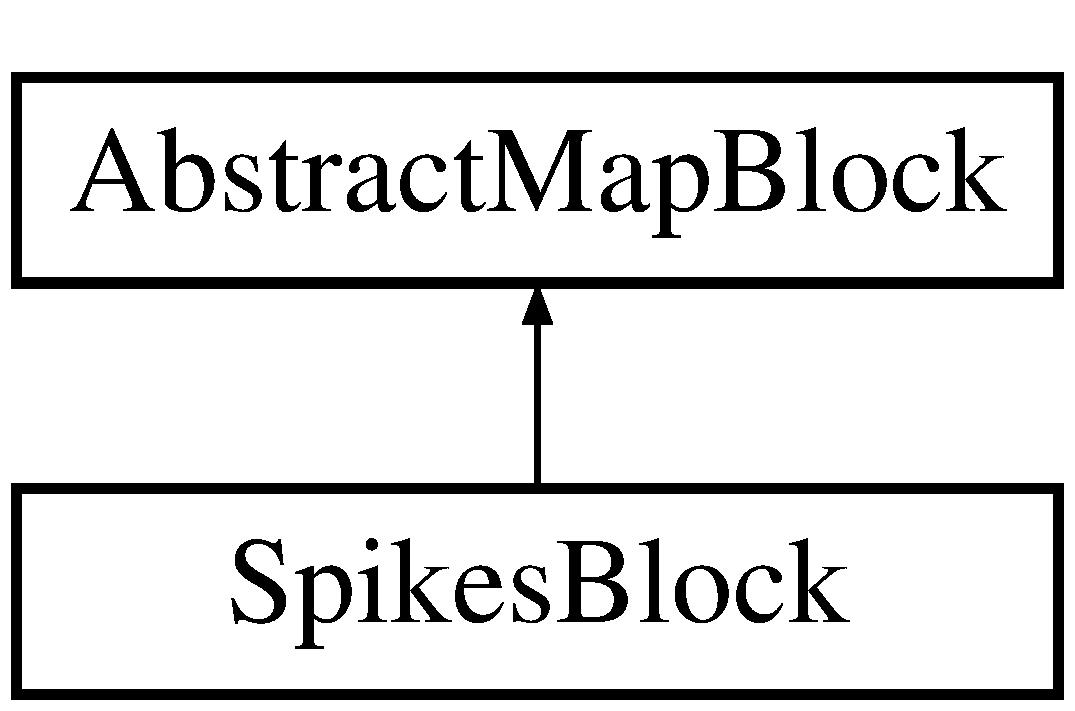
\includegraphics[height=2.000000cm]{class_spikes_block}
\end{center}
\end{figure}
\subsection*{Public Member Functions}
\begin{DoxyCompactItemize}
\item 
\mbox{\Hypertarget{class_spikes_block_ae1ae23307e042a765a02bcf208df00a6}\label{class_spikes_block_ae1ae23307e042a765a02bcf208df00a6}} 
{\bfseries Spikes\+Block} (int x, int y)
\item 
\mbox{\Hypertarget{class_spikes_block_a01ee14c5a7053180abfc6620fbe1e3cd}\label{class_spikes_block_a01ee14c5a7053180abfc6620fbe1e3cd}} 
sf\+::\+Sprite $\ast$ {\bfseries get\+Sprite} ()
\end{DoxyCompactItemize}
\subsection*{Protected Attributes}
\begin{DoxyCompactItemize}
\item 
\mbox{\Hypertarget{class_spikes_block_a0280cf45f757b2bf74f06394d7c51d28}\label{class_spikes_block_a0280cf45f757b2bf74f06394d7c51d28}} 
sf\+::\+Texture $\ast$ {\bfseries texture}
\item 
\mbox{\Hypertarget{class_spikes_block_af553d7cee5570d44b0352a583e348a77}\label{class_spikes_block_af553d7cee5570d44b0352a583e348a77}} 
sf\+::\+Sprite $\ast$ {\bfseries sprite}
\end{DoxyCompactItemize}
\subsection*{Additional Inherited Members}


The documentation for this class was generated from the following files\+:\begin{DoxyCompactItemize}
\item 
Spikes\+Block.\+h\item 
Spikes\+Block.\+cpp\end{DoxyCompactItemize}

\hypertarget{class_stone_block}{}\section{Stone\+Block Class Reference}
\label{class_stone_block}\index{Stone\+Block@{Stone\+Block}}
Inheritance diagram for Stone\+Block\+:\begin{figure}[H]
\begin{center}
\leavevmode
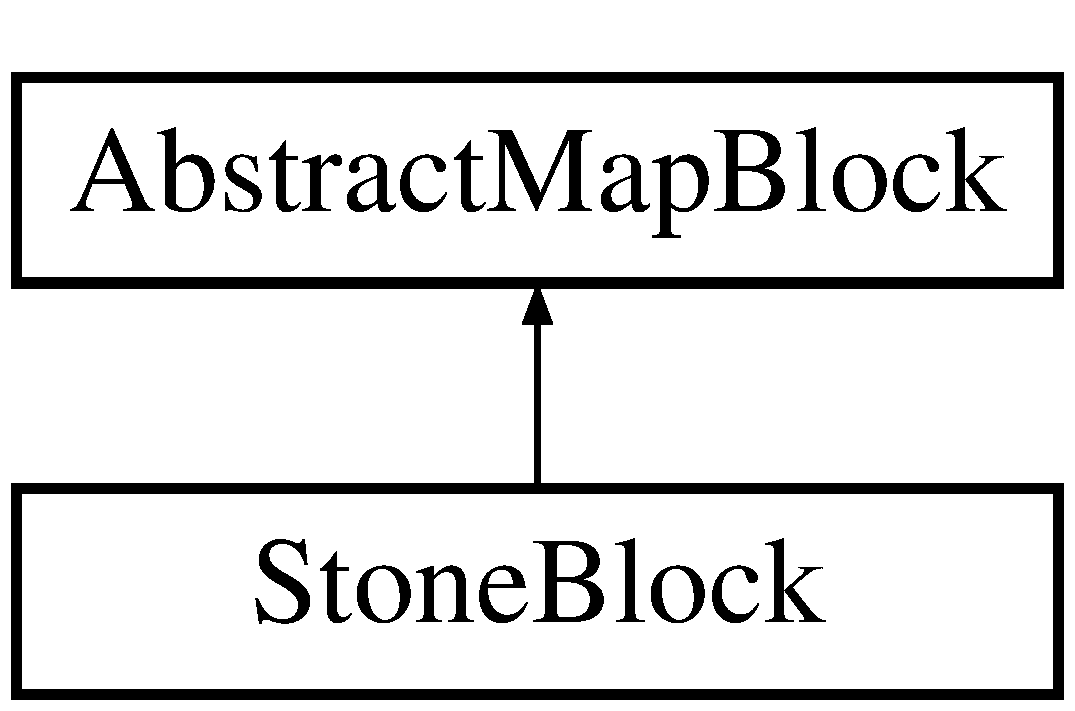
\includegraphics[height=2.000000cm]{class_stone_block}
\end{center}
\end{figure}
\subsection*{Public Member Functions}
\begin{DoxyCompactItemize}
\item 
\mbox{\Hypertarget{class_stone_block_aa2e4adb1d50d9f326ffe427bcdd6d7bb}\label{class_stone_block_aa2e4adb1d50d9f326ffe427bcdd6d7bb}} 
sf\+::\+Sprite $\ast$ {\bfseries get\+Sprite} ()
\item 
\mbox{\Hypertarget{class_stone_block_a391e99e613d1864c93647f60c9455a74}\label{class_stone_block_a391e99e613d1864c93647f60c9455a74}} 
void {\bfseries constructor} ()
\end{DoxyCompactItemize}
\subsection*{Protected Attributes}
\begin{DoxyCompactItemize}
\item 
\mbox{\Hypertarget{class_stone_block_a86062896e0fedaad3bedbbd52641f76b}\label{class_stone_block_a86062896e0fedaad3bedbbd52641f76b}} 
sf\+::\+Texture $\ast$ {\bfseries texture}
\item 
\mbox{\Hypertarget{class_stone_block_a1d66339d3e42126e72130dd6863d30b5}\label{class_stone_block_a1d66339d3e42126e72130dd6863d30b5}} 
sf\+::\+Sprite $\ast$ {\bfseries sprite}
\end{DoxyCompactItemize}
\subsection*{Additional Inherited Members}


The documentation for this class was generated from the following files\+:\begin{DoxyCompactItemize}
\item 
Stone\+Block.\+h\item 
Stone\+Block.\+cpp\end{DoxyCompactItemize}

\chapter{File Documentation}
\hypertarget{_abstract_map_block_8cpp}{}\section{Abstract\+Map\+Block.\+cpp File Reference}
\label{_abstract_map_block_8cpp}\index{Abstract\+Map\+Block.\+cpp@{Abstract\+Map\+Block.\+cpp}}
{\ttfamily \#include \char`\"{}stdafx.\+h\char`\"{}}\newline
{\ttfamily \#include \char`\"{}Abstract\+Map\+Block.\+h\char`\"{}}\newline

\hypertarget{_abstract_map_block_8h}{}\section{Abstract\+Map\+Block.\+h File Reference}
\label{_abstract_map_block_8h}\index{Abstract\+Map\+Block.\+h@{Abstract\+Map\+Block.\+h}}
{\ttfamily \#include $<$S\+F\+M\+L/\+Graphics.\+hpp$>$}\newline
\subsection*{Classes}
\begin{DoxyCompactItemize}
\item 
class \hyperlink{class_abstract_map_block}{Abstract\+Map\+Block}
\end{DoxyCompactItemize}

\hypertarget{_block_8cpp}{}\section{Block.\+cpp File Reference}
\label{_block_8cpp}\index{Block.\+cpp@{Block.\+cpp}}
{\ttfamily \#include \char`\"{}stdafx.\+h\char`\"{}}\newline
{\ttfamily \#include \char`\"{}Block.\+h\char`\"{}}\newline
{\ttfamily \#include $<$S\+F\+M\+L/\+Graphics.\+hpp$>$}\newline

\hypertarget{_block_8h}{}\section{Block.\+h File Reference}
\label{_block_8h}\index{Block.\+h@{Block.\+h}}
{\ttfamily \#include \char`\"{}Abstract\+Map\+Block.\+h\char`\"{}}\newline
\subsection*{Classes}
\begin{DoxyCompactItemize}
\item 
class \hyperlink{class_block}{Block}
\end{DoxyCompactItemize}

\hypertarget{_bridge_block_8cpp}{}\section{Bridge\+Block.\+cpp File Reference}
\label{_bridge_block_8cpp}\index{Bridge\+Block.\+cpp@{Bridge\+Block.\+cpp}}
{\ttfamily \#include \char`\"{}stdafx.\+h\char`\"{}}\newline
{\ttfamily \#include \char`\"{}Bridge\+Block.\+h\char`\"{}}\newline

\hypertarget{_bridge_block_8h}{}\section{Bridge\+Block.\+h File Reference}
\label{_bridge_block_8h}\index{Bridge\+Block.\+h@{Bridge\+Block.\+h}}
{\ttfamily \#include \char`\"{}Abstract\+Map\+Block.\+h\char`\"{}}\newline
\subsection*{Classes}
\begin{DoxyCompactItemize}
\item 
class \hyperlink{class_bridge_block}{Bridge\+Block}
\end{DoxyCompactItemize}

\hypertarget{_bush_block_8cpp}{}\section{Bush\+Block.\+cpp File Reference}
\label{_bush_block_8cpp}\index{Bush\+Block.\+cpp@{Bush\+Block.\+cpp}}
{\ttfamily \#include \char`\"{}stdafx.\+h\char`\"{}}\newline
{\ttfamily \#include \char`\"{}Bush\+Block.\+h\char`\"{}}\newline

\hypertarget{_bush_block_8h}{}\section{Bush\+Block.\+h File Reference}
\label{_bush_block_8h}\index{Bush\+Block.\+h@{Bush\+Block.\+h}}
{\ttfamily \#include \char`\"{}Abstract\+Map\+Block.\+h\char`\"{}}\newline
\subsection*{Classes}
\begin{DoxyCompactItemize}
\item 
class \hyperlink{class_bush_block}{Bush\+Block}
\end{DoxyCompactItemize}

\hypertarget{c2_project_8cpp}{}\section{c2\+Project.\+cpp File Reference}
\label{c2_project_8cpp}\index{c2\+Project.\+cpp@{c2\+Project.\+cpp}}
{\ttfamily \#include \char`\"{}stdafx.\+h\char`\"{}}\newline
{\ttfamily \#include $<$S\+F\+M\+L/\+Graphics.\+hpp$>$}\newline
{\ttfamily \#include $<$S\+F\+M\+L/\+Audio.\+hpp$>$}\newline
{\ttfamily \#include \char`\"{}Map.\+h\char`\"{}}\newline
{\ttfamily \#include \char`\"{}Gravity.\+h\char`\"{}}\newline
\subsection*{Functions}
\begin{DoxyCompactItemize}
\item 
int \hyperlink{c2_project_8cpp_ae66f6b31b5ad750f1fe042a706a4e3d4}{main} ()
\end{DoxyCompactItemize}


\subsection{Function Documentation}
\mbox{\Hypertarget{c2_project_8cpp_ae66f6b31b5ad750f1fe042a706a4e3d4}\label{c2_project_8cpp_ae66f6b31b5ad750f1fe042a706a4e3d4}} 
\index{c2\+Project.\+cpp@{c2\+Project.\+cpp}!main@{main}}
\index{main@{main}!c2\+Project.\+cpp@{c2\+Project.\+cpp}}
\subsubsection{\texorpdfstring{main()}{main()}}
{\footnotesize\ttfamily int main (\begin{DoxyParamCaption}{ }\end{DoxyParamCaption})}


\hypertarget{_character_8cpp}{}\section{Character.\+cpp File Reference}
\label{_character_8cpp}\index{Character.\+cpp@{Character.\+cpp}}
{\ttfamily \#include \char`\"{}stdafx.\+h\char`\"{}}\newline
{\ttfamily \#include \char`\"{}Character.\+h\char`\"{}}\newline
{\ttfamily \#include $<$S\+F\+M\+L/\+Graphics.\+hpp$>$}\newline
{\ttfamily \#include $<$iostream$>$}\newline

\hypertarget{_character_8h}{}\section{Character.\+h File Reference}
\label{_character_8h}\index{Character.\+h@{Character.\+h}}
{\ttfamily \#include $<$S\+F\+M\+L/\+Graphics.\+hpp$>$}\newline
\subsection*{Classes}
\begin{DoxyCompactItemize}
\item 
class \hyperlink{class_character}{Character}
\end{DoxyCompactItemize}

\hypertarget{_crate_block_8cpp}{}\section{Crate\+Block.\+cpp File Reference}
\label{_crate_block_8cpp}\index{Crate\+Block.\+cpp@{Crate\+Block.\+cpp}}
{\ttfamily \#include \char`\"{}stdafx.\+h\char`\"{}}\newline
{\ttfamily \#include \char`\"{}Crate\+Block.\+h\char`\"{}}\newline

\hypertarget{_crate_block_8h}{}\section{Crate\+Block.\+h File Reference}
\label{_crate_block_8h}\index{Crate\+Block.\+h@{Crate\+Block.\+h}}
{\ttfamily \#include \char`\"{}Abstract\+Map\+Block.\+h\char`\"{}}\newline
\subsection*{Classes}
\begin{DoxyCompactItemize}
\item 
class \hyperlink{class_crate_block}{Crate\+Block}
\end{DoxyCompactItemize}

\hypertarget{_display_map_manager_8cpp}{}\section{Display\+Map\+Manager.\+cpp File Reference}
\label{_display_map_manager_8cpp}\index{Display\+Map\+Manager.\+cpp@{Display\+Map\+Manager.\+cpp}}
{\ttfamily \#include \char`\"{}stdafx.\+h\char`\"{}}\newline
{\ttfamily \#include \char`\"{}Display\+Map\+Manager.\+h\char`\"{}}\newline
{\ttfamily \#include \char`\"{}Map.\+h\char`\"{}}\newline
{\ttfamily \#include $<$S\+F\+M\+L/\+Graphics.\+hpp$>$}\newline
{\ttfamily \#include \char`\"{}Stone\+Block.\+h\char`\"{}}\newline
{\ttfamily \#include $<$S\+F\+M\+L/\+Audio.\+hpp$>$}\newline
{\ttfamily \#include $<$windows.\+h$>$}\newline
{\ttfamily \#include $<$string$>$}\newline

\hypertarget{_display_map_manager_8h}{}\section{Display\+Map\+Manager.\+h File Reference}
\label{_display_map_manager_8h}\index{Display\+Map\+Manager.\+h@{Display\+Map\+Manager.\+h}}
{\ttfamily \#include \char`\"{}Map.\+h\char`\"{}}\newline
{\ttfamily \#include $<$S\+F\+M\+L/\+Graphics.\+hpp$>$}\newline
\subsection*{Classes}
\begin{DoxyCompactItemize}
\item 
class \hyperlink{class_display_map_manager}{Display\+Map\+Manager}
\end{DoxyCompactItemize}
\subsection*{Macros}
\begin{DoxyCompactItemize}
\item 
\#define \hyperlink{_display_map_manager_8h_a2beea3dee2937ac69773a3591b58e884}{W\+I\+N\+D\+O\+W\+S\+\_\+\+W\+I\+D\+TH}~1920
\item 
\#define \hyperlink{_display_map_manager_8h_ac2792af9d84f5421586a955baee972c4}{W\+I\+N\+D\+O\+W\+S\+\_\+\+H\+E\+I\+G\+HT}~1080
\end{DoxyCompactItemize}


\subsection{Macro Definition Documentation}
\mbox{\Hypertarget{_display_map_manager_8h_ac2792af9d84f5421586a955baee972c4}\label{_display_map_manager_8h_ac2792af9d84f5421586a955baee972c4}} 
\index{Display\+Map\+Manager.\+h@{Display\+Map\+Manager.\+h}!W\+I\+N\+D\+O\+W\+S\+\_\+\+H\+E\+I\+G\+HT@{W\+I\+N\+D\+O\+W\+S\+\_\+\+H\+E\+I\+G\+HT}}
\index{W\+I\+N\+D\+O\+W\+S\+\_\+\+H\+E\+I\+G\+HT@{W\+I\+N\+D\+O\+W\+S\+\_\+\+H\+E\+I\+G\+HT}!Display\+Map\+Manager.\+h@{Display\+Map\+Manager.\+h}}
\subsubsection{\texorpdfstring{W\+I\+N\+D\+O\+W\+S\+\_\+\+H\+E\+I\+G\+HT}{WINDOWS\_HEIGHT}}
{\footnotesize\ttfamily \#define W\+I\+N\+D\+O\+W\+S\+\_\+\+H\+E\+I\+G\+HT~1080}

\mbox{\Hypertarget{_display_map_manager_8h_a2beea3dee2937ac69773a3591b58e884}\label{_display_map_manager_8h_a2beea3dee2937ac69773a3591b58e884}} 
\index{Display\+Map\+Manager.\+h@{Display\+Map\+Manager.\+h}!W\+I\+N\+D\+O\+W\+S\+\_\+\+W\+I\+D\+TH@{W\+I\+N\+D\+O\+W\+S\+\_\+\+W\+I\+D\+TH}}
\index{W\+I\+N\+D\+O\+W\+S\+\_\+\+W\+I\+D\+TH@{W\+I\+N\+D\+O\+W\+S\+\_\+\+W\+I\+D\+TH}!Display\+Map\+Manager.\+h@{Display\+Map\+Manager.\+h}}
\subsubsection{\texorpdfstring{W\+I\+N\+D\+O\+W\+S\+\_\+\+W\+I\+D\+TH}{WINDOWS\_WIDTH}}
{\footnotesize\ttfamily \#define W\+I\+N\+D\+O\+W\+S\+\_\+\+W\+I\+D\+TH~1920}


\hypertarget{_gravity_8cpp}{}\section{Gravity.\+cpp File Reference}
\label{_gravity_8cpp}\index{Gravity.\+cpp@{Gravity.\+cpp}}
{\ttfamily \#include \char`\"{}stdafx.\+h\char`\"{}}\newline
{\ttfamily \#include \char`\"{}Gravity.\+h\char`\"{}}\newline
{\ttfamily \#include $<$S\+F\+M\+L/\+Audio.\+hpp$>$}\newline

\hypertarget{_gravity_8h}{}\section{Gravity.\+h File Reference}
\label{_gravity_8h}\index{Gravity.\+h@{Gravity.\+h}}
{\ttfamily \#include \char`\"{}Display\+Map\+Manager.\+h\char`\"{}}\newline
{\ttfamily \#include $<$S\+F\+M\+L/\+Audio.\+hpp$>$}\newline
\subsection*{Classes}
\begin{DoxyCompactItemize}
\item 
class \hyperlink{class_gravity}{Gravity}
\end{DoxyCompactItemize}
\subsection*{Macros}
\begin{DoxyCompactItemize}
\item 
\#define \hyperlink{_gravity_8h_a7f79c5b3e28385fc1da3bfd61668bff7}{G\+R\+A\+V\+I\+T\+Y\+\_\+\+S\+T\+A\+T\+U\+S\+\_\+\+N\+O\+R\+M\+AL}~0
\item 
\#define \hyperlink{_gravity_8h_adde6d741afb9f6d8ece6c2eca45497e6}{G\+R\+A\+V\+I\+T\+Y\+\_\+\+S\+T\+A\+T\+U\+S\+\_\+\+J\+U\+MP}~10
\item 
\#define \hyperlink{_gravity_8h_acbc668496ad78b72d72c15fba994847f}{G\+R\+A\+V\+I\+T\+Y\+\_\+\+S\+T\+A\+T\+U\+S\+\_\+\+F\+A\+LL}~20
\end{DoxyCompactItemize}


\subsection{Macro Definition Documentation}
\mbox{\Hypertarget{_gravity_8h_acbc668496ad78b72d72c15fba994847f}\label{_gravity_8h_acbc668496ad78b72d72c15fba994847f}} 
\index{Gravity.\+h@{Gravity.\+h}!G\+R\+A\+V\+I\+T\+Y\+\_\+\+S\+T\+A\+T\+U\+S\+\_\+\+F\+A\+LL@{G\+R\+A\+V\+I\+T\+Y\+\_\+\+S\+T\+A\+T\+U\+S\+\_\+\+F\+A\+LL}}
\index{G\+R\+A\+V\+I\+T\+Y\+\_\+\+S\+T\+A\+T\+U\+S\+\_\+\+F\+A\+LL@{G\+R\+A\+V\+I\+T\+Y\+\_\+\+S\+T\+A\+T\+U\+S\+\_\+\+F\+A\+LL}!Gravity.\+h@{Gravity.\+h}}
\subsubsection{\texorpdfstring{G\+R\+A\+V\+I\+T\+Y\+\_\+\+S\+T\+A\+T\+U\+S\+\_\+\+F\+A\+LL}{GRAVITY\_STATUS\_FALL}}
{\footnotesize\ttfamily \#define G\+R\+A\+V\+I\+T\+Y\+\_\+\+S\+T\+A\+T\+U\+S\+\_\+\+F\+A\+LL~20}

\mbox{\Hypertarget{_gravity_8h_adde6d741afb9f6d8ece6c2eca45497e6}\label{_gravity_8h_adde6d741afb9f6d8ece6c2eca45497e6}} 
\index{Gravity.\+h@{Gravity.\+h}!G\+R\+A\+V\+I\+T\+Y\+\_\+\+S\+T\+A\+T\+U\+S\+\_\+\+J\+U\+MP@{G\+R\+A\+V\+I\+T\+Y\+\_\+\+S\+T\+A\+T\+U\+S\+\_\+\+J\+U\+MP}}
\index{G\+R\+A\+V\+I\+T\+Y\+\_\+\+S\+T\+A\+T\+U\+S\+\_\+\+J\+U\+MP@{G\+R\+A\+V\+I\+T\+Y\+\_\+\+S\+T\+A\+T\+U\+S\+\_\+\+J\+U\+MP}!Gravity.\+h@{Gravity.\+h}}
\subsubsection{\texorpdfstring{G\+R\+A\+V\+I\+T\+Y\+\_\+\+S\+T\+A\+T\+U\+S\+\_\+\+J\+U\+MP}{GRAVITY\_STATUS\_JUMP}}
{\footnotesize\ttfamily \#define G\+R\+A\+V\+I\+T\+Y\+\_\+\+S\+T\+A\+T\+U\+S\+\_\+\+J\+U\+MP~10}

\mbox{\Hypertarget{_gravity_8h_a7f79c5b3e28385fc1da3bfd61668bff7}\label{_gravity_8h_a7f79c5b3e28385fc1da3bfd61668bff7}} 
\index{Gravity.\+h@{Gravity.\+h}!G\+R\+A\+V\+I\+T\+Y\+\_\+\+S\+T\+A\+T\+U\+S\+\_\+\+N\+O\+R\+M\+AL@{G\+R\+A\+V\+I\+T\+Y\+\_\+\+S\+T\+A\+T\+U\+S\+\_\+\+N\+O\+R\+M\+AL}}
\index{G\+R\+A\+V\+I\+T\+Y\+\_\+\+S\+T\+A\+T\+U\+S\+\_\+\+N\+O\+R\+M\+AL@{G\+R\+A\+V\+I\+T\+Y\+\_\+\+S\+T\+A\+T\+U\+S\+\_\+\+N\+O\+R\+M\+AL}!Gravity.\+h@{Gravity.\+h}}
\subsubsection{\texorpdfstring{G\+R\+A\+V\+I\+T\+Y\+\_\+\+S\+T\+A\+T\+U\+S\+\_\+\+N\+O\+R\+M\+AL}{GRAVITY\_STATUS\_NORMAL}}
{\footnotesize\ttfamily \#define G\+R\+A\+V\+I\+T\+Y\+\_\+\+S\+T\+A\+T\+U\+S\+\_\+\+N\+O\+R\+M\+AL~0}


\hypertarget{_ground_block_8cpp}{}\section{Ground\+Block.\+cpp File Reference}
\label{_ground_block_8cpp}\index{Ground\+Block.\+cpp@{Ground\+Block.\+cpp}}
{\ttfamily \#include \char`\"{}stdafx.\+h\char`\"{}}\newline
{\ttfamily \#include \char`\"{}Ground\+Block.\+h\char`\"{}}\newline
{\ttfamily \#include $<$S\+F\+M\+L/\+Graphics.\+hpp$>$}\newline

\hypertarget{_ground_block_8h}{}\section{Ground\+Block.\+h File Reference}
\label{_ground_block_8h}\index{Ground\+Block.\+h@{Ground\+Block.\+h}}
{\ttfamily \#include \char`\"{}Abstract\+Map\+Block.\+h\char`\"{}}\newline
\subsection*{Classes}
\begin{DoxyCompactItemize}
\item 
class \hyperlink{class_ground_block}{Ground\+Block}
\end{DoxyCompactItemize}

\hypertarget{_map_8cpp}{}\section{Map.\+cpp File Reference}
\label{_map_8cpp}\index{Map.\+cpp@{Map.\+cpp}}
{\ttfamily \#include \char`\"{}stdafx.\+h\char`\"{}}\newline
{\ttfamily \#include \char`\"{}Map.\+h\char`\"{}}\newline
{\ttfamily \#include \char`\"{}Stone\+Block.\+h\char`\"{}}\newline
{\ttfamily \#include \char`\"{}Block.\+h\char`\"{}}\newline
{\ttfamily \#include \char`\"{}Ground\+Block.\+h\char`\"{}}\newline
{\ttfamily \#include \char`\"{}Plank\+Block.\+h\char`\"{}}\newline
{\ttfamily \#include \char`\"{}Bridge\+Block.\+h\char`\"{}}\newline
{\ttfamily \#include \char`\"{}Crate\+Block.\+h\char`\"{}}\newline
{\ttfamily \#include \char`\"{}Spikes\+Block.\+h\char`\"{}}\newline
{\ttfamily \#include \char`\"{}Bush\+Block.\+h\char`\"{}}\newline
{\ttfamily \#include $<$iostream$>$}\newline

\hypertarget{_map_8h}{}\section{Map.\+h File Reference}
\label{_map_8h}\index{Map.\+h@{Map.\+h}}
{\ttfamily \#include \char`\"{}Character.\+h\char`\"{}}\newline
{\ttfamily \#include $<$S\+F\+M\+L/\+Graphics.\+hpp$>$}\newline
{\ttfamily \#include $<$list$>$}\newline
{\ttfamily \#include \char`\"{}Stone\+Block.\+h\char`\"{}}\newline
\subsection*{Classes}
\begin{DoxyCompactItemize}
\item 
class \hyperlink{class_map}{Map}
\end{DoxyCompactItemize}

\hypertarget{_plank_block_8cpp}{}\section{Plank\+Block.\+cpp File Reference}
\label{_plank_block_8cpp}\index{Plank\+Block.\+cpp@{Plank\+Block.\+cpp}}
{\ttfamily \#include \char`\"{}stdafx.\+h\char`\"{}}\newline
{\ttfamily \#include \char`\"{}Plank\+Block.\+h\char`\"{}}\newline

\hypertarget{_plank_block_8h}{}\section{Plank\+Block.\+h File Reference}
\label{_plank_block_8h}\index{Plank\+Block.\+h@{Plank\+Block.\+h}}
{\ttfamily \#include \char`\"{}Abstract\+Map\+Block.\+h\char`\"{}}\newline
\subsection*{Classes}
\begin{DoxyCompactItemize}
\item 
class \hyperlink{class_plank_block}{Plank\+Block}
\end{DoxyCompactItemize}

\hypertarget{resource_8h}{}\section{resource.\+h File Reference}
\label{resource_8h}\index{resource.\+h@{resource.\+h}}

\hypertarget{_spikes_block_8cpp}{}\section{Spikes\+Block.\+cpp File Reference}
\label{_spikes_block_8cpp}\index{Spikes\+Block.\+cpp@{Spikes\+Block.\+cpp}}
{\ttfamily \#include \char`\"{}stdafx.\+h\char`\"{}}\newline
{\ttfamily \#include \char`\"{}Spikes\+Block.\+h\char`\"{}}\newline

\hypertarget{_spikes_block_8h}{}\section{Spikes\+Block.\+h File Reference}
\label{_spikes_block_8h}\index{Spikes\+Block.\+h@{Spikes\+Block.\+h}}
{\ttfamily \#include \char`\"{}Abstract\+Map\+Block.\+h\char`\"{}}\newline
\subsection*{Classes}
\begin{DoxyCompactItemize}
\item 
class \hyperlink{class_spikes_block}{Spikes\+Block}
\end{DoxyCompactItemize}

\hypertarget{stdafx_8cpp}{}\section{stdafx.\+cpp File Reference}
\label{stdafx_8cpp}\index{stdafx.\+cpp@{stdafx.\+cpp}}
{\ttfamily \#include \char`\"{}stdafx.\+h\char`\"{}}\newline

\hypertarget{stdafx_8h}{}\section{stdafx.\+h File Reference}
\label{stdafx_8h}\index{stdafx.\+h@{stdafx.\+h}}
{\ttfamily \#include \char`\"{}targetver.\+h\char`\"{}}\newline
{\ttfamily \#include $<$stdio.\+h$>$}\newline
{\ttfamily \#include $<$tchar.\+h$>$}\newline

\hypertarget{_stone_block_8cpp}{}\section{Stone\+Block.\+cpp File Reference}
\label{_stone_block_8cpp}\index{Stone\+Block.\+cpp@{Stone\+Block.\+cpp}}
{\ttfamily \#include \char`\"{}stdafx.\+h\char`\"{}}\newline
{\ttfamily \#include \char`\"{}Stone\+Block.\+h\char`\"{}}\newline
{\ttfamily \#include $<$S\+F\+M\+L/\+Graphics.\+hpp$>$}\newline

\hypertarget{_stone_block_8h}{}\section{Stone\+Block.\+h File Reference}
\label{_stone_block_8h}\index{Stone\+Block.\+h@{Stone\+Block.\+h}}
{\ttfamily \#include \char`\"{}Abstract\+Map\+Block.\+h\char`\"{}}\newline
{\ttfamily \#include $<$S\+F\+M\+L/\+Graphics.\+hpp$>$}\newline
\subsection*{Classes}
\begin{DoxyCompactItemize}
\item 
class \hyperlink{class_stone_block}{Stone\+Block}
\end{DoxyCompactItemize}

\hypertarget{targetver_8h}{}\section{targetver.\+h File Reference}
\label{targetver_8h}\index{targetver.\+h@{targetver.\+h}}
{\ttfamily \#include $<$S\+D\+K\+D\+D\+K\+Ver.\+h$>$}\newline

%--- End generated contents ---

% Index
\backmatter
\newpage
\phantomsection
\clearemptydoublepage
\addcontentsline{toc}{chapter}{Index}
\printindex

\end{document}
